\documentclass[12pt,a4paper]{report}

% ---------- Core packages (XeLaTeX: native Unicode + system fonts, needed to
% typeset the real Bangla-script queries this report quotes as evidence) ----------
\usepackage{fontspec}
\usepackage[a4paper,left=1.35in,right=1in,top=1.1in,bottom=1.1in]{geometry}
% Fonts are embedded as files in fonts/ (not looked up by OS font name) so
% this compiles identically on Overleaf (Linux) as on any local machine --
% TeX Gyre Termes is a free, metric-compatible Times clone; Noto Sans
% Bengali (SIL OFL) covers the Bangla-script queries quoted in this report.
\setmainfont{texgyretermes}[
  Extension = .otf,
  UprightFont = *-regular,
  BoldFont = *-bold,
  ItalicFont = *-italic,
  BoldItalicFont = *-bolditalic,
  Path = fonts/,
]
\newfontfamily\bengalifont{NotoSansBengali}[
  Extension = .ttf,
  UprightFont = *-Regular,
  BoldFont = *-Bold,
  Path = fonts/,
]
\newcommand{\bn}[1]{{\bengalifont #1}}
\usepackage{microtype}
\usepackage{graphicx}
\usepackage{xcolor}
\usepackage{titlesec}
\usepackage{fancyhdr}
\usepackage{booktabs}
\usepackage{array}
\usepackage{longtable}
\usepackage{enumitem}
\usepackage{setspace}
\usepackage{hyperref}
\usepackage{float}
\usepackage{amssymb}
\usepackage{caption}
\usepackage[titles]{tocloft}

% ---------- Brand colours (match the app + slide deck) ----------
\definecolor{brandprimary}{HTML}{0E7C86}
\definecolor{branddark}{HTML}{0B4F57}
\definecolor{brandgray}{HTML}{374151}
\definecolor{codebg}{HTML}{F1F8F8}
\definecolor{codeink}{HTML}{0B4F57}

\hypersetup{
    colorlinks=true, linkcolor=branddark, citecolor=branddark, urlcolor=brandprimary,
    pdftitle={ShopMate AI -- Project Book},
    pdfauthor={Tanvir Ahmed},
    bookmarksopen=true, bookmarksnumbered=true,
}

\titleformat{\chapter}[display]
  {\normalfont\Huge\bfseries\color{branddark}}
  {\filright\Large\MakeUppercase{\chaptertitlename}~\thechapter}
  {6pt}{\Large}
\titlespacing*{\chapter}{0pt}{-10pt}{28pt}
\titleformat{\section}{\normalfont\Large\bfseries\color{branddark}}{\thesection}{0.6em}{}
\titleformat{\subsection}{\normalfont\large\bfseries\color{brandgray}}{\thesubsection}{0.6em}{}
\titlespacing*{\section}{0pt}{16pt}{6pt}
\titlespacing*{\subsection}{0pt}{10pt}{4pt}

\renewcommand{\cftchapfont}{\bfseries\color{branddark}}
\renewcommand{\cftchappagefont}{\color{branddark}}
\renewcommand{\cftsecfont}{\color{brandgray}}

\pagestyle{fancy}
\fancyhf{}
\setlength{\headheight}{14pt}
\renewcommand{\headrulewidth}{0.4pt}
\fancyhead[L]{\small\itshape ShopMate AI --- Project Book}
\fancyhead[R]{\small\itshape Tanvir Ahmed}
\fancyfoot[C]{\thepage}
\fancypagestyle{plain}{\fancyhf{}\fancyfoot[C]{\thepage}\renewcommand{\headrulewidth}{0pt}}

\graphicspath{{figures/}}
\setstretch{1.15}
\emergencystretch=3em
\tolerance=1200
\hbadness=10000
\captionsetup{font=small,labelfont={bf,color=branddark},skip=6pt}

% ---------- code listing box (identifiers/snippets) ----------
\newcommand{\codebox}[1]{%
  \par\noindent\colorbox{codebg}{%
    \begin{minipage}{\dimexpr\linewidth-2\fboxsep}
      \ttfamily\small\color{codeink}
      #1
    \end{minipage}%
  }\par\vspace{6pt}
}

\setlist[itemize]{leftmargin=1.3cm, itemsep=3pt, topsep=4pt}

\begin{document}

% ============================================================
% TITLE PAGE
% ============================================================
\begin{titlepage}
\centering
\vspace*{0.4cm}
{\bfseries\fontsize{15}{18}\selectfont\color{branddark} Mawlana Bhashani Science and Technology University}\\[4pt]
{\small Santosh, Tangail-1902, Bangladesh}\\[6pt]
{\bfseries\fontsize{12.5}{15}\selectfont Department of Information and Communication Technology}\\[30pt]

{\color{brandprimary}\rule{0.82\textwidth}{1pt}}\\[9pt]
{\bfseries\fontsize{17}{20}\selectfont\color{branddark} PROJECT BOOK}\\[9pt]
{\color{brandprimary}\rule{0.82\textwidth}{1pt}}\\[26pt]

{\small Submitted in partial fulfilment of the requirements for the degree of}\\[4pt]
{\bfseries\fontsize{12.5}{15}\selectfont Master of Engineering in Information and Communication Technology}\\[36pt]

{\bfseries\fontsize{28}{32}\selectfont\color{brandprimary} ShopMate AI}\\[14pt]
\begin{minipage}{0.82\textwidth}
\centering
{\bfseries\fontsize{14}{18}\selectfont Design and Development of an LLM-Orchestrated, Retrieval-Augmented
Conversational Agent for Cross-Platform Product Discovery, Semantic Product Matching and Personalized
E-Commerce Recommendation\par}
\end{minipage}\\[40pt]

\begin{minipage}{0.42\textwidth}
\centering
\small\textbf{Submitted by}\\[6pt]
\normalsize\textbf{Tanvir Ahmed}\\
\small Student ID: IT22604\\
M.Engineering (ICT)
\end{minipage}%
\begin{minipage}{0.42\textwidth}
\centering
\small\textbf{Submitted to}\\[6pt]
\normalsize\textbf{Nazrul Islam}\\
\small Associate Professor\\
Department of ICT\\
MBSTU
\end{minipage}

\vfill
{\normalsize\itshape August 2026}
\end{titlepage}

\pagenumbering{roman}

% ============================================================
\chapter*{Declaration}
\addcontentsline{toc}{chapter}{Declaration}
I hereby declare that this project book, titled ``ShopMate AI: Design and Development of an
LLM-Orchestrated, Retrieval-Augmented Conversational Agent for Cross-Platform Product Discovery, Semantic
Product Matching and Personalized E-Commerce Recommendation,'' is my own original work, carried out under
the supervision of Nazrul Islam, Associate Professor, Department of ICT, Mawlana Bhashani Science and
Technology University. All architectural decisions, source code, evaluation design, and results reported
in this book were produced by me for this project and have not been submitted, in whole or in part, for
any other degree or qualification at this or any other institution. Where the work of others has been
consulted, drawn upon, or cited, it has been explicitly acknowledged in the References.

\vspace{3cm}
\noindent
\begin{minipage}{0.48\textwidth}
\_\_\_\_\_\_\_\_\_\_\_\_\_\_\_\_\_\_\_\_\_\_\_\_\_\_\\
Tanvir Ahmed\\
Student ID: IT22604
\end{minipage}%
\hfill
\begin{minipage}{0.42\textwidth}
\raggedleft
Date: 31 August 2026
\end{minipage}

% ============================================================
\chapter*{Certificate}
\addcontentsline{toc}{chapter}{Certificate}
This is to certify that the project book titled ``ShopMate AI: Design and Development of an
LLM-Orchestrated, Retrieval-Augmented Conversational Agent for Cross-Platform Product Discovery, Semantic
Product Matching and Personalized E-Commerce Recommendation'' has been carried out by Tanvir Ahmed
(Student ID: IT22604) under my supervision, in partial fulfilment of the requirements for the degree of
Master of Engineering in Information and Communication Technology at Mawlana Bhashani Science and
Technology University. To the best of my knowledge, the work reported here is original and has not been
submitted elsewhere for the award of any other degree.

\vspace{3.5cm}
\noindent
\_\_\_\_\_\_\_\_\_\_\_\_\_\_\_\_\_\_\_\_\_\_\_\_\_\_\\
Nazrul Islam\\
Associate Professor, Department of ICT\\
Mawlana Bhashani Science and Technology University\\
Supervisor

% ============================================================
\chapter*{Acknowledgement}
\addcontentsline{toc}{chapter}{Acknowledgement}
I would like to express my sincere gratitude to my supervisor, Nazrul Islam, Associate Professor,
Department of ICT, Mawlana Bhashani Science and Technology University, for his continuous guidance,
constructive feedback, and encouragement throughout the design, development, and evaluation of this
project. I am also grateful to the faculty members of the Department of ICT for the foundation of
knowledge on which this work builds, and to my family and peers for their patience and support during the
course of this project.

% ============================================================
\chapter*{Abstract}
\addcontentsline{toc}{chapter}{Abstract}
Online shopping across multiple Bangladeshi e-commerce platforms forces a buyer to repeat the same search
on every site and manually reconcile price, delivery cost, and rating differences by hand. Conventional
keyword search compounds this: it cannot resolve constraint-rich natural-language requests such as
``a black backpack under BDT 3,000 with a laptop compartment,'' and it does not understand Bangla or
code-mixed Banglish queries at all. This project presents ShopMate AI, a conversational shopping agent
that separates natural-language query understanding from product retrieval and ranking through a
service-oriented architecture: a Laravel (PHP) application owns authentication, orders, and the
administrative dashboard, while a Python FastAPI service performs intent classification, entity
extraction, hybrid keyword/TF-IDF retrieval, and multi-factor ranking. Query understanding is
dual-pipeline --- a deterministic, whole-word rule-based extractor is always available, and an optional
OpenAI-compatible LLM backend can replace it, with every LLM field independently re-validated against the
same closed vocabulary the rule-based path already trusts, and an unconditional fallback to the rule-based
pipeline on any failure. A cross-store product-matching service resolves the same physical product listed
under different titles across stores using token-set Jaccard similarity over normalized titles, a
brand-conflict veto, and a model-code veto, so that price, delivery, and rating can be compared
like-for-like rather than as unrelated listings. When a query returns zero local results, an on-demand
live-search fallback queries a real external catalogue (Othoba.com), ingests any genuine matches into the
local catalogue through the same matching service, and retries the search once --- without a second
language-understanding round trip. All purchase actions require explicit human confirmation before an
order is recorded; no automated checkout, CAPTCHA bypass, or payment action is performed. The system was
evaluated against a conventional keyword-search baseline on eleven hand-labelled queries spanning budget,
brand, attribute, multi-constraint, and Bangla/Banglish categories, measuring Precision@5, Recall@5, and
NDCG@5. ShopMate AI achieved Recall@5~=~1.00 and NDCG@5~=~1.00 against the baseline's 0.59 and 0.59, and
the baseline scored exactly zero on every budget-aware, multi-constraint, and Bangla/Banglish query in the
set --- precisely the category of query a keyword index cannot resolve. The report documents the system's
architecture, algorithms, a real engineering case study in calibrating a semantic-trust threshold, the
evaluation methodology and results, and the limitations and future work that follow from a TF-IDF-based,
single-machine implementation.

\vspace{10pt}
\noindent\textbf{Keywords:} Conversational commerce, retrieval-augmented search, large language models,
intent classification, entity extraction, TF-IDF, hybrid retrieval, cross-store product matching,
learning-to-rank, Bangla/Banglish natural language processing.

% ============================================================
\tableofcontents
\listoffigures
\listoftables

\cleardoublepage
\pagenumbering{arabic}

% ============================================================
% CHAPTER 1
% ============================================================
\chapter{Introduction}

\section{Background}
Online shopping in Bangladesh, as elsewhere, has grown into a fragmented experience. A buyer who wants a
single product --- a backpack, a phone, a kitchen appliance --- often has to open several e-commerce sites,
repeat the same search on each, and manually compare price, delivery cost, seller reliability and reviews
before deciding where to buy. Native site search on each of these platforms is keyword-driven: it matches
the literal words in a query against product titles and returns an unranked or popularity-ranked list,
leaving all of the comparison work to the buyer.

Two further gaps compound this problem. First, constraint-rich, natural requests such as ``a black
backpack under BDT 3,000 that can carry both a laptop and clothes'' are handled poorly by keyword search,
because a keyword index has no way to reason about a numeric budget constraint or a colour attribute
jointly with a category. Second, a large share of real shopping queries in Bangladesh are expressed in
Bangla script or in Banglish (Bangla transliterated into Latin characters, sometimes mixed with English),
and conventional search boxes built for English keyword matching frequently fail to understand them at
all.

\section{Motivation}
Recent progress in transformer-based language understanding and large language models (LLMs) has made it
practical to build a conversational agent that extracts structured shopping requirements from free-form,
multilingual text. At the same time, classical information-retrieval techniques such as TF-IDF weighting
and cosine similarity remain a lightweight, dependency-light way to rank textual relevance without
requiring a GPU or a large embedding model --- an important constraint for a project that must run on
ordinary development hardware. This project is motivated by the gap between what buyers actually want to
say (``cheap phone under 22000 taka'', \bn{কালো ব্যাগ}) and what conventional shopping interfaces are able
to understand, and by the opportunity to close that gap with a hybrid design: a deterministic rule-based
baseline for reliability, an optional LLM backend for genuine language understanding, and classical
retrieval and ranking underneath both.

\section{Problem Statement}
The absence of a conversational, cross-platform shopping agent leaves buyers in Bangladesh without:
\begin{itemize}
\item A single interface through which a natural-language or Bangla/Banglish shopping request can be
understood and acted on, rather than re-typed as isolated keywords on every store's own search box;
\item An automated way to identify the same or an equivalent product listed under different titles and
descriptions across stores, so that price and delivery can be compared like-for-like;
\item A structured, explainable comparison of price, delivery cost, rating and availability across
supported stores, with a stated reason for why a particular option is recommended;
\item A mechanism to be notified when a tracked product's price drops, a desired item is restocked, or a
searched-for product that was not available becomes available; and
\item A human-confirmed, safe purchase-recording workflow rather than either fully manual shopping or
unsupervised automated checkout that bypasses a store's own authentication or payment controls.
\end{itemize}

\section{Objectives}
\subsection{General Objective}
To design, implement, and evaluate a modular, LLM-orchestrated, retrieval-augmented conversational
shopping agent that understands natural-language (including Bangla/Banglish) shopping requests, searches a
multi-store product catalogue through hybrid keyword and TF-IDF retrieval, performs cross-store product
matching, generates personalized, explainable recommendations via a multi-factor ranking model, extends
coverage through on-demand live search, and supports a human-confirmed purchase-recording workflow.

\subsection{Specific Objectives}
\begin{itemize}
\item Design a service-oriented architecture that separates business logic (Laravel/PHP) from AI/NLP
processing (a Python FastAPI service).
\item Implement a dual-pipeline intent-classification and entity-extraction system: a deterministic
rule-based extractor always available, and an optional LLM backend for genuine natural-language and
Bangla/Banglish understanding, with mandatory graceful degradation on failure.
\item Build a hybrid keyword-filtered and TF-IDF relevance retrieval pipeline over a normalized,
multi-store product catalogue, and calibrate a relevance floor that rejects coincidental word overlap
without rejecting genuine matches.
\item Implement a cross-store, dependency-free product-matching service so that the same or an equivalent
product listed under different titles is correctly identified, merged, and compared, while never merging
listings from clearly different named brands or conflicting model codes.
\item Implement an explainable, multi-factor ranking engine that combines relevance, price, rating,
delivery cost and availability, with a stated reason for each recommendation.
\item Implement an on-demand live-search fallback that extends catalogue coverage to a real external store
when a query returns zero local results, and permanently ingests genuine matches for future queries.
\item Implement price-drop alerting, a shopping-list module, and a pre-order/notify-me queue for demand the
current catalogue cannot satisfy.
\item Implement a human-confirmed order-recording workflow that never places or pays for anything on a
store's own site and never bypasses authentication, CAPTCHA or payment controls.
\item Evaluate the system experimentally against a conventional keyword-search baseline using Precision@5,
Recall@5 and NDCG@5 over a hand-labelled, multi-category query set.
\end{itemize}

\section{Scope of the Project}
The delivered system covers conversational product discovery, cross-store comparison, explainable
recommendation, price-drop and stock alerting, a shopping list, and a human-confirmed order-recording
workflow, built as a modular web application (Laravel + Python FastAPI AI service) over a mock multi-store
catalogue plus one real live integration (Othoba.com, used strictly through its public, search-only API).
The following are explicitly out of scope for this delivery: fully automated purchase execution without
human confirmation; voice shopping and image-based visual product search; SMS gateway integration; and
coverage of more than a small number of store integrations. Automated bypass of CAPTCHA, authentication,
anti-bot measures, or payment security is excluded from the design at every stage --- the system never
submits a real order to a store, only records a user's confirmed intent and links out to the store's own
listing.

\section{Report Organization}
Chapter~2 reviews existing approaches to e-commerce search, price comparison, and conversational commerce,
and positions this project against that background. Chapter~3 analyzes the functional and non-functional
requirements the system must satisfy. Chapter~4 presents the system design: the layered architecture,
technology stack, database design, and the cross-store matching design. Chapter~5 describes the
implementation of the query-understanding, retrieval, ranking, live-fallback, and order-confirmation
components, including a worked engineering case study. Chapter~6 presents the evaluation methodology and
results against a keyword-search baseline. Chapter~7 walks through the working system with screenshots
from the running application. Chapter~8 concludes with a summary of contributions, limitations, and future
work.

% ============================================================
% CHAPTER 2
% ============================================================
\chapter{Literature Review}

\section{Conventional E-Commerce Search}
The dominant search paradigm on individual e-commerce platforms is inverted-index keyword matching,
typically backed by engines such as Elasticsearch or a platform-specific search service, ranked by a
mixture of textual relevance and business signals such as popularity or sponsorship. This approach is well
understood and fast, but it is fundamentally single-platform: it has no notion of a product listed on a
competing store, and it treats a query as a bag of words rather than a set of structured constraints. A
query such as ``under 3000 taka'' is, to a pure keyword index, just three more tokens to match against
product titles rather than a numeric filter to apply.

\section{Price-Comparison Platforms}
Third-party price-comparison sites address the multi-store gap by aggregating listings, but the matching
between listings is typically manually curated or updated on a slow batch cycle, and the query interface
remains keyword-based. None of the reviewed approaches address Bangla or Banglish input, and none combine
comparison with a conversational interface that can parse multi-constraint natural-language requests.

\section{Conversational Commerce and Large Language Models}
Transformer-based language models \cite{devlin2019,reimers2019} established that pretrained contextual
representations dramatically improve natural-language understanding tasks such as intent classification
and named-entity extraction over hand-written rules. Instruction-tuned large language models extend this
further: a general-purpose LLM can be prompted, without task-specific fine-tuning, to extract structured
fields (category, brand, budget, colour) from a free-form sentence in any language it has been trained on,
including code-mixed Bangla/Banglish. Published conversational-commerce research, however, largely targets
English-only, single-market catalogues, and typically assumes the LLM's output can be trusted directly
rather than treating it as a hypothesis that must be corroborated or safely rejected. This project treats
an LLM-supplied category specifically as a hypothesis: Sections~5.2 and~6.5 describe a real failure mode
this assumption caused, and the corroboration mechanism built to fix it.

\section{Information Retrieval Foundations}
Term Frequency-Inverse Document Frequency (TF-IDF) weighting combined with cosine similarity
\cite{manning2008} remains a strong, well-understood baseline for text relevance ranking: it requires no
training data, no GPU, and no large model download, at the cost of being a purely lexical signal with no
semantic generalization --- it cannot on its own recognise that ``earphone'' and ``earbuds'' refer to the
same product category, or that a Bangla-script query and an English-titled catalogue describe the same
product. Dense sentence embeddings \cite{reimers2019} address the semantic-generalization gap at the cost
of a heavier runtime dependency (a transformer encoder). This project uses TF-IDF as the retrieval-scoring
layer specifically to keep the AI service free of a torch/transformers dependency and runnable on ordinary
development hardware, and compensates for its lexical blind spots with a structured-entity filter layer
and a synonym dictionary that a rule-based or LLM-based understanding stage can draw on --- the documented
upgrade path to sentence-transformer embeddings, once the lexical ceiling is reached, is recorded in the
project's implementation notes.

\section{Cross-Store Product Matching}
Matching product records across independently authored catalogues is a recognised entity-resolution
problem: different stores title, describe, and structure the same physical product differently, and a
naive text-similarity match is vulnerable to both false negatives (genuinely equivalent products with very
different phrasing) and false positives (different products that happen to share templated marketing
boilerplate, e.g. two unrelated phones both titled ``... (Best Price) (Original)''). Model-based
entity-resolution approaches exist, but add a training and inference dependency; this project instead uses
a dependency-free, tunable heuristic --- token-set Jaccard similarity over normalized, stop-worded titles,
an exact-brand-conflict veto, and a model/variant-code veto --- described fully in Section~4.5, chosen so
that matching stays fast and auditable on real, messy listing data rather than only on a clean hand-built
fixture.

\section{Research Gap and Positioning}
Taken together, native site search is keyword-only and single-platform; price-comparison sites are
manually curated and not conversational; and published conversational-commerce research largely targets
English-only, single-market settings and trusts LLM output without independent corroboration. This project
is positioned to close that specific, compound gap: a conversational agent that combines dual-pipeline
intent/entity extraction (rule-based with an optional, independently-validated LLM backend), TF-IDF hybrid
retrieval with a calibrated relevance floor, dependency-free cross-store product matching, and explainable
multi-factor ranking --- evaluated specifically on Bangla/Banglish and multi-constraint shopping queries
against a conventional keyword-search baseline, which Chapter~6 shows scores exactly zero on precisely
that category of query.

% ============================================================
% CHAPTER 3
% ============================================================
\chapter{System Analysis and Requirements}

\section{Functional Requirements}
\begin{longtable}{p{1.3cm}p{11.7cm}}
\toprule
\textbf{ID} & \textbf{Requirement} \\
\midrule
\endfirsthead
\toprule
\textbf{ID} & \textbf{Requirement} \\
\midrule
\endhead
FR-1 & The system shall allow a user to register, log in, and manage a profile. \\
FR-2 & The system shall accept a shopping request as a free-form chat message in English, Bangla, or
Banglish, within a persisted conversation. \\
FR-3 & The system shall classify the message's intent (e.g. SEARCH\_PRODUCT, RECOMMEND\_PRODUCT,
PRICE\_ALERT, STOCK\_ALERT, SHOPPING\_LIST, BUY\_PRODUCT) and extract structured entities (category,
brand, colour, budget, rating threshold, delivery preference). \\
FR-4 & The system shall retrieve matching products from a multi-store catalogue using both structured
filters and text relevance, and shall return no results rather than an unrelated result set when nothing
genuinely matches. \\
FR-5 & The system shall identify equivalent products listed under different titles across stores and
present them as one comparable product with multiple offers. \\
FR-6 & The system shall rank matching products using relevance, price, rating, delivery cost and
availability, and shall state a reason for each ranked result. \\
FR-7 & When a query returns zero local results, the system shall attempt a live search against a real
external store, ingest genuine matches into the local catalogue, and retry the search once. \\
FR-8 & The system shall let a user create price-drop and restock alerts, and a shopping list, for products
or search terms. \\
FR-9 & When a searched-for product is not available anywhere, the system shall let the user register a
pre-order/notify-me request. \\
FR-10 & The system shall require explicit human confirmation before recording any order, and shall never
submit an order or payment to a store's own site. \\
FR-11 & The system shall provide an administrative dashboard summarizing store health, product counts,
users, and search activity. \\
FR-12 & The system shall let a user opt in or out of including international-origin stores in search
results. \\
\bottomrule
\caption{Functional requirements.}
\end{longtable}

\section{Non-Functional Requirements}
\begin{longtable}{p{1.4cm}p{5.5cm}p{5.6cm}}
\toprule
\textbf{ID} & \textbf{Requirement} & \textbf{Rationale} \\
\midrule
\endfirsthead
\toprule
\textbf{ID} & \textbf{Requirement} & \textbf{Rationale} \\
\midrule
\endhead
NFR-1 & The AI service shall run without a GPU or large model download. & Must run on ordinary
development/lab hardware. \\
NFR-2 & Query understanding shall degrade gracefully to a deterministic pipeline on any external LLM
failure. & An optional network dependency must never take the whole chat feature down. \\
NFR-3 & A search that resolves to zero genuine matches shall return an empty result, never an unrelated
one. & Trust and usefulness of recommendations depend on this. \\
NFR-4 & Two listings from clearly different named brands shall never be auto-merged into one product. &
A wrong merge silently corrupts the price comparison for both products. \\
NFR-5 & No component shall bypass a store's authentication, CAPTCHA, or payment controls. & Ethical/legal
boundary stated in the project's scope. \\
NFR-6 & The chat UI shall visibly indicate when a response is being generated. & A multi-hundred-
millisecond to multi-second round trip must not read as an unresponsive page. \\
NFR-7 & The system shall be deployable on Windows (XAMPP/MySQL) or Linux development environments. &
Matches the actual development and demonstration environment. \\
\bottomrule
\caption{Non-functional requirements.}
\end{longtable}

\section{Actors and Use Cases}
Two actors interact with the system: the shopper, who converses with the assistant, manages a shopping
list and alerts, and confirms orders; and the administrator, who reviews store health, product data
quality, and search analytics from the admin dashboard. The shopper's central use case --- ``search for a
product in natural language and receive a ranked, explainable, cross-store comparison'' --- is the one
this report evaluates in Chapter~6, and it decomposes into the query-understanding, retrieval, matching,
and ranking responsibilities detailed in Chapter~5.

\section{Feasibility}
Technical feasibility rests on three deliberately lightweight choices, each made to keep the system
runnable on a single low-spec machine without a dedicated inference server: TF-IDF instead of a
sentence-embedding model for retrieval scoring (Section~2.4); a dependency-free heuristic instead of a
trained entity-resolution model for cross-store matching (Section~2.5); and a rule-based extractor that
remains fully functional with the LLM backend disabled (Sections~5.1--5.2). Economic feasibility is
supported by the same choices: the only paid dependency is the optional LLM API call, which the system is
designed to function correctly without. Operational feasibility follows from the human-confirmed order
workflow (Section~5.6), which keeps the system within a safe, non-transactional scope that requires no
payment-processing compliance.

% ============================================================
% CHAPTER 4
% ============================================================
\chapter{System Design}

\section{Architectural Overview}
ShopMate AI follows a layered, service-oriented architecture that isolates AI/NLP processing from core
business logic, shown in Figure~\ref{fig:arch}. The Laravel application owns authentication, user data,
conversations, orders, and the administrative dashboard; it communicates with the Python AI service over
an internal HTTP API for intent detection, entity extraction, retrieval, and ranking. This separation means
the AI service can be developed, tested, and evaluated (Chapter~6) independently of the web application,
and that the retrieval/ranking algorithms have no dependency on PHP or Laravel at all.

\begin{figure}[H]
\centering
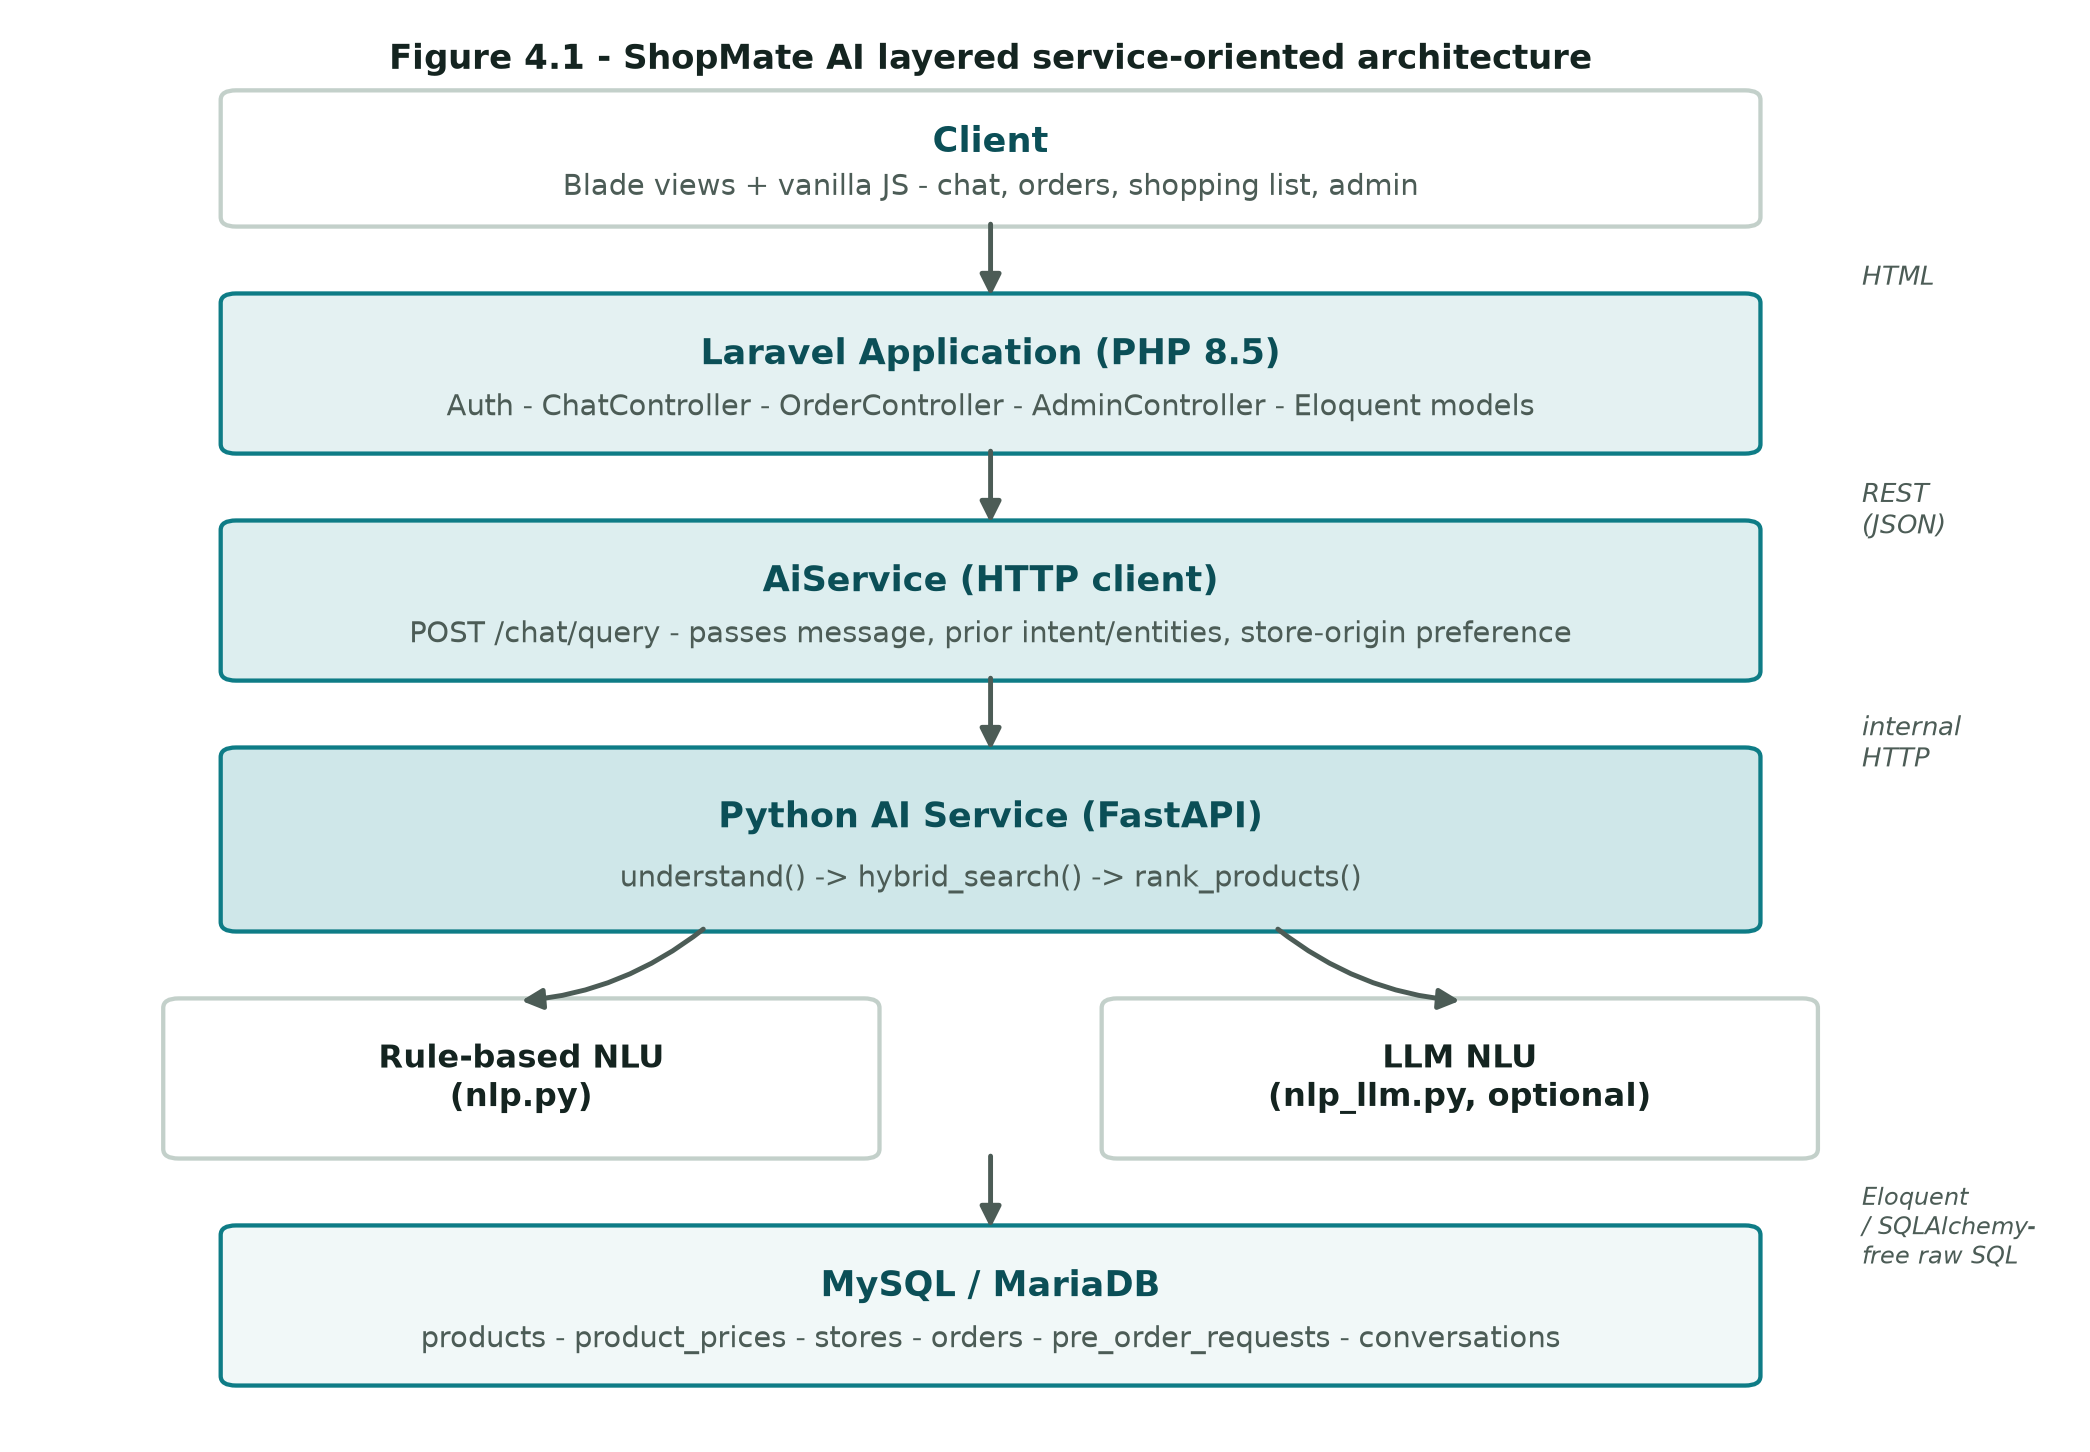
\includegraphics[width=0.92\textwidth]{fig_architecture.png}
\caption{ShopMate AI layered service-oriented architecture.}
\label{fig:arch}
\end{figure}

\section{Technology Stack}
\begin{table}[H]
\centering
\small
\begin{tabular}{p{2.6cm}p{4.6cm}p{5.6cm}}
\toprule
\textbf{Layer} & \textbf{Technology} & \textbf{Notes} \\
\midrule
Backend application & Laravel 13 (PHP 8.5) & Auth, conversations, orders, alerts, shopping list, admin
dashboard \\
Frontend & Blade views + vanilla JavaScript & Server-rendered UI; JS handles chat loading state and
auto-scroll \\
AI service & Python 3.13 + FastAPI & Stateless HTTP service; one endpoint, \texttt{POST /chat/query} \\
Query understanding & Rule-based + optional LLM & OpenAI-compatible chat-completions API;
deepseek-v4-flash used in evaluation runs \\
Retrieval & scikit-learn \texttt{TfidfVectorizer} + cosine similarity & No torch/transformers dependency \\
Cross-store matching & Custom PHP service (token-set Jaccard) & No ML model; dependency-free \\
Database & MySQL / MariaDB (via XAMPP in development) & Shared by both services; AI service reads with
raw SQL \\
Live external data & Othoba.com public Typesense search API & Search-only key; used only for on-demand
fallback, never for checkout \\
Deployment (dev) & Windows + XAMPP (MySQL) + standalone PHP 8.5 + Python venv & \texttt{start.bat} /
\texttt{start.ps1} launch both services together \\
\bottomrule
\end{tabular}
\caption{Technology stack actually used in the implementation.}
\end{table}

\section{Database Design}
The relational schema separates a canonical, store-independent product record from its per-store
listings, which is what makes cross-store comparison possible: one \texttt{products} row can have many
\texttt{product\_prices} rows, one per store that carries it. Table~\ref{tab:db} summarises the principal
tables.

\begin{longtable}{p{3.4cm}p{5.0cm}p{4.4cm}}
\caption{Principal database tables.}\label{tab:db} \\
\toprule
\textbf{Table} & \textbf{Purpose} & \textbf{Key columns} \\
\midrule
\endfirsthead
\toprule
\textbf{Table} & \textbf{Purpose} & \textbf{Key columns} \\
\midrule
\endhead
\texttt{users} & Accounts and preferences & \texttt{is\_admin}, \texttt{include\_international\_stores} \\
\texttt{stores} & Store registry & \texttt{name}, \texttt{origin} (domestic / international) \\
\texttt{products} & Canonical, store-independent product & \texttt{canonical\_title}, \texttt{category},
\texttt{brand}, \texttt{attributes} (JSON) \\
\texttt{product\_prices} & One store's listing of a product & \texttt{product\_id}, \texttt{store\_id},
\texttt{price}, \texttt{delivery\_charge}, \texttt{rating}, \texttt{in\_stock}, \texttt{product\_url} \\
\texttt{possible\_duplicate\_products} & Queue of matches below the auto-merge threshold & reviewed
manually by an admin \\
\texttt{conversations} / \texttt{messages} & Chat history & \texttt{conversation\_id}, \texttt{role},
\texttt{body}, \texttt{intent}, \texttt{entities} (JSON) \\
\texttt{search\_history} & Logged queries & query text, resolved intent/entities \\
\texttt{shopping\_lists} / \texttt{shopping\_list\_items} & Recurring-purchase lists & quantity, target
product/category \\
\texttt{price\_alerts} & Price-drop / restock subscriptions & \texttt{product\_id},
\texttt{threshold\_price} \\
\texttt{pre\_order\_requests} & Demand for a query that matched nothing & \texttt{query},
\texttt{category}, \texttt{brand}, \texttt{user\_id} \\
\texttt{orders} & Human-confirmed order records & \texttt{status} (\texttt{confirmed\_redirected} /
\texttt{cancelled}), \texttt{product\_url} \\
\bottomrule
\end{longtable}

\noindent Every \texttt{product\_prices} row retains the store's own \texttt{product\_url} and raw
\texttt{store\_title}, preserving traceability back to the originating listing even after several stores'
listings have been merged under one canonical product.

\section{Store Provider Abstraction}
Every data source --- the seeded mock domestic stores, the live Othoba.com integration, and a mock
international store (GlobalDeals Express) --- implements a common \texttt{StoreProviderInterface} exposing
\texttt{slug()}, \texttt{name()}, \texttt{origin()} (domestic or international), and
\texttt{fetchListings()}, which returns raw listings in one normalized shape (title, price,
delivery\_charge, rating, review\_count, in\_stock, brand, category, description, attributes). Nothing
downstream --- matching, search, or ranking --- needs to know which kind of provider a listing came from.
Adding a new store means implementing one interface against the existing pipeline, not modifying it.

\section{Cross-Store Product Matching Design}
The matching design's central risk is asymmetric: failing to merge two listings of the same product only
costs a slightly less complete comparison, but wrongly merging two different products silently corrupts
the price comparison for both, in a way a user has no way to detect. The design in Figure~\ref{fig:match}
is therefore deliberately conservative --- two vetoes can force outright rejection before any similarity
score is even consulted:
\begin{itemize}
\item \textbf{Brand-conflict veto}: if both the incoming listing and a candidate product have a named
brand and the names differ, similarity is forced to 0.0 regardless of how similar the titles read.
\item \textbf{Model-code veto}: if both titles contain a letters-then-digits variant code (e.g. ``a17'',
``s24'') and none of the listing's codes match any of the candidate's, similarity is forced to 0.0 ---
this specifically catches same-brand, different-model confusions such as ``Samsung Galaxy A17'' vs.
``Samsung Galaxy A07''.
\end{itemize}

\noindent Past both vetoes, similarity is token-set Jaccard overlap between stop-worded, normalized
titles, boosted by 0.30 when both sides share a known brand. The auto-merge threshold is 0.65 when a brand
is known on both sides, but raised to 0.80 when neither side has a usable brand --- generic, unbranded
listings (cables, screen protectors, umbrellas) were found during tuning to share so much templated
marketing boilerplate that plain title overlap alone could clear a lower threshold despite being different
products. A pair that clears its threshold is merged as another offer on the existing product; otherwise a
new canonical product is created.

\begin{figure}[H]
\centering
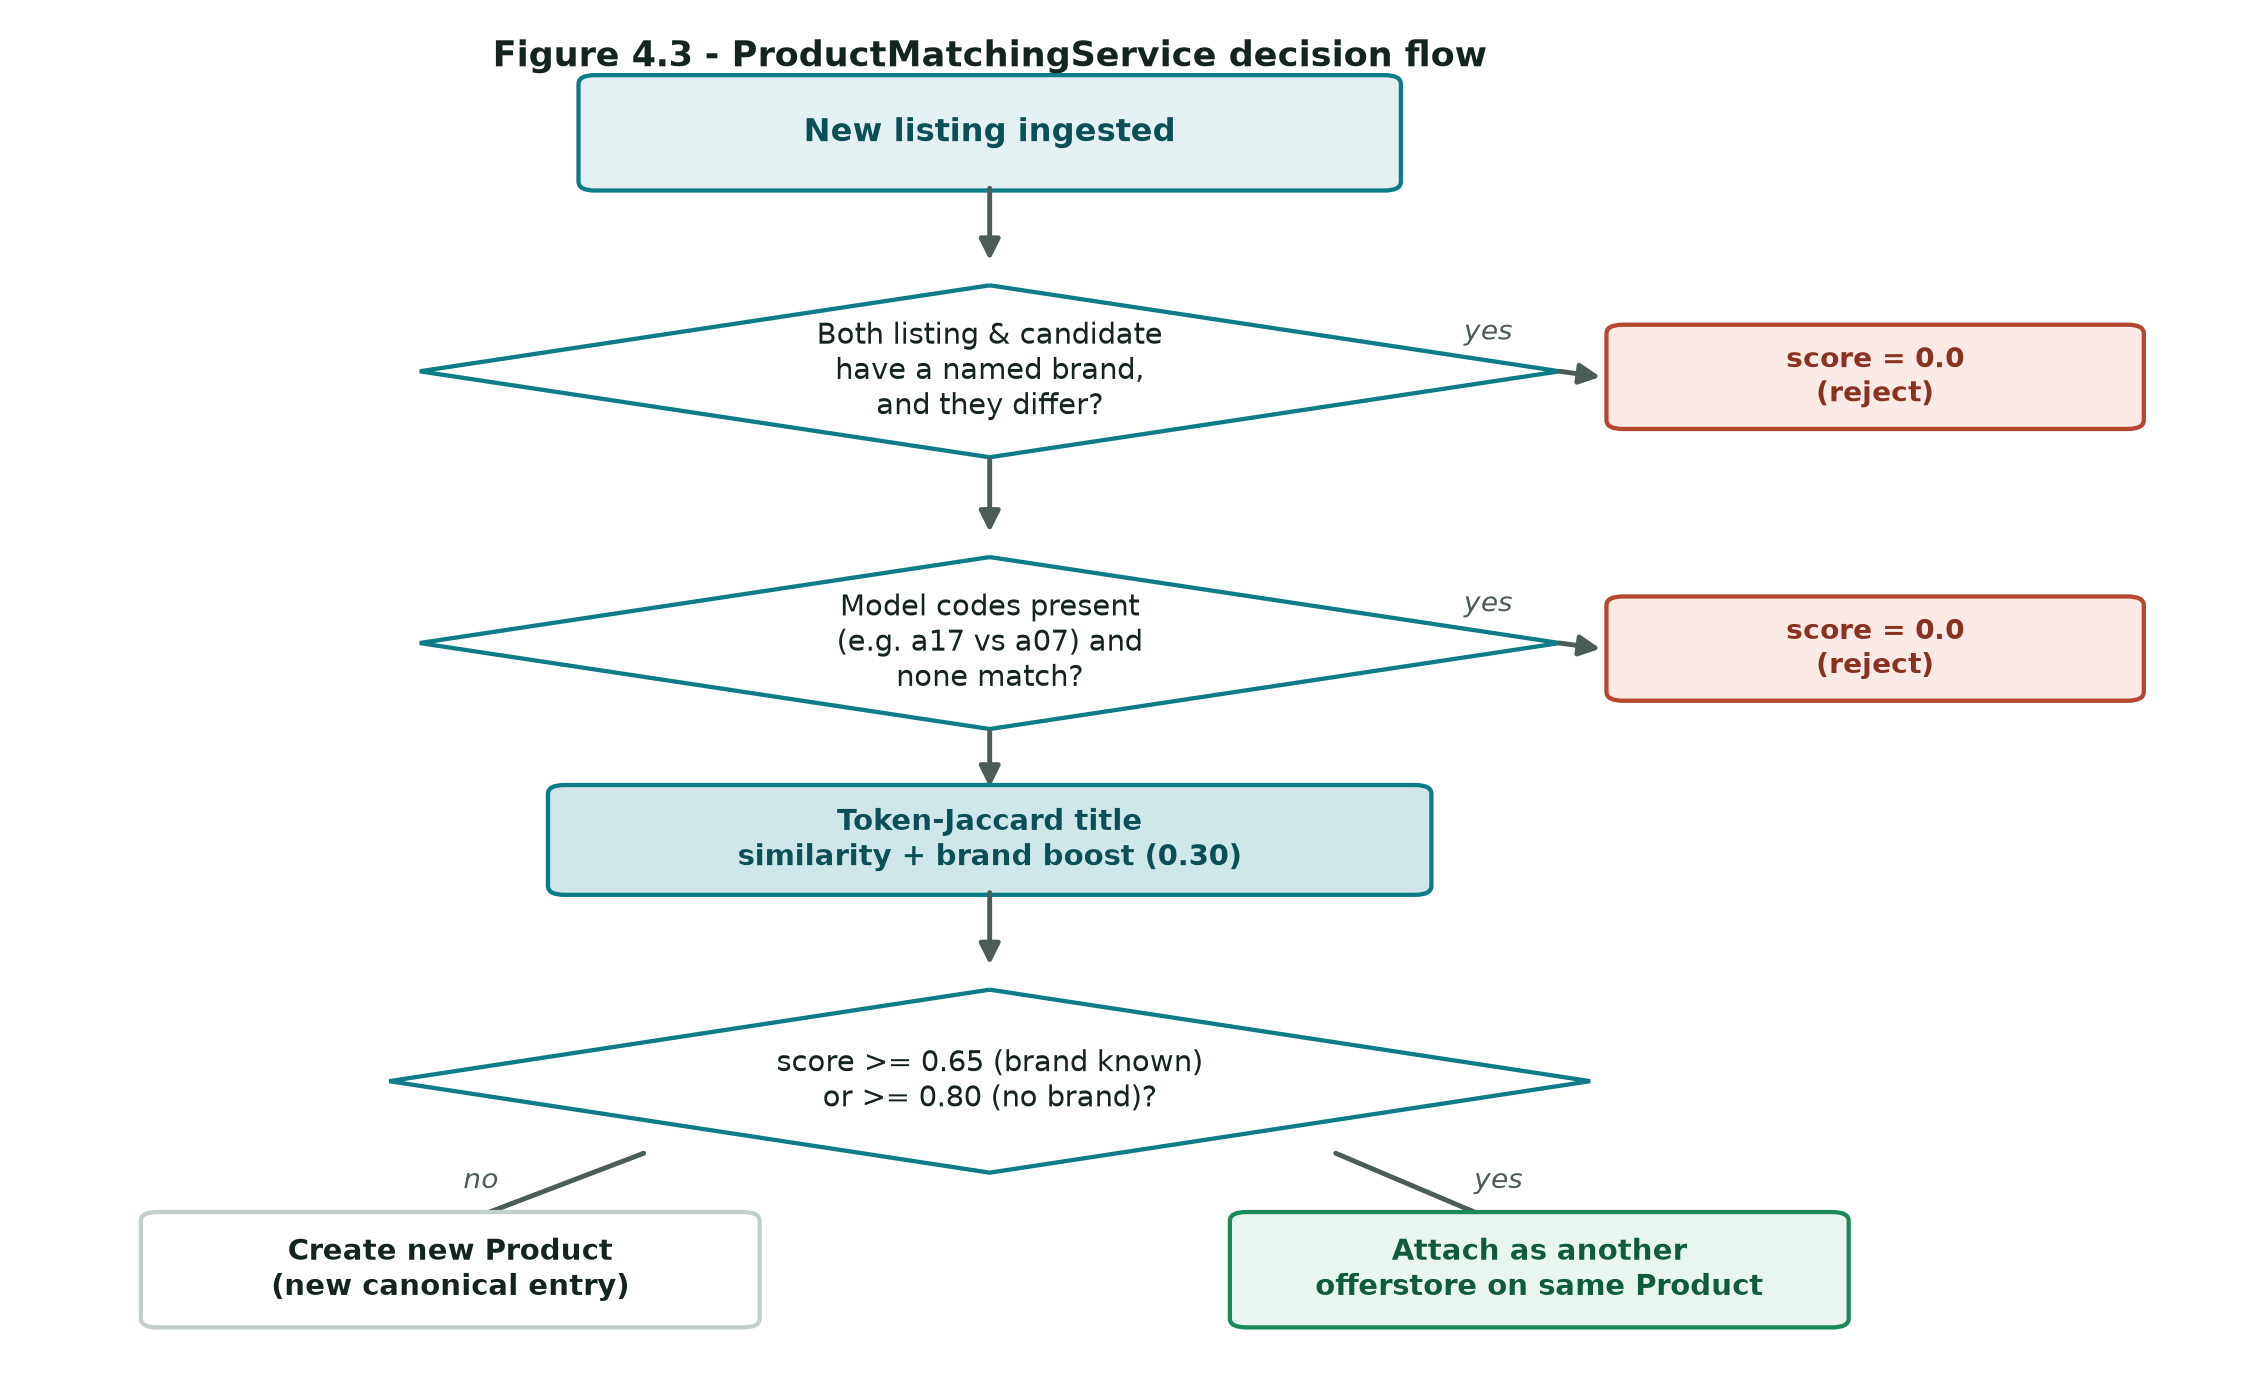
\includegraphics[width=0.78\textwidth]{fig_matching.png}
\caption{ProductMatchingService decision flow.}
\label{fig:match}
\end{figure}

\noindent This design was tuned against two different datasets on purpose: a clean, hand-crafted
three-store mock fixture, and real listings pulled live from Othoba.com. The mock fixture alone hid a real
precision bug --- on real data, two genuinely different phones (``Samsung Galaxy A17'' and ``Samsung
Galaxy A07'') scored above an earlier, lower auto-merge threshold purely on brand match plus generic
shared words (``galaxy'', ``ram'', ``rom''). The model-code veto exists specifically to fix that case
without regressing the mock fixture's validated 100\% recall.

% ============================================================
% CHAPTER 5
% ============================================================
\chapter{Implementation}

This chapter follows one query end to end through the four stages shown in Figure~\ref{fig:pipeline}, then
describes the live-fallback and human-confirmed order features that sit around that core loop.

\begin{figure}[H]
\centering
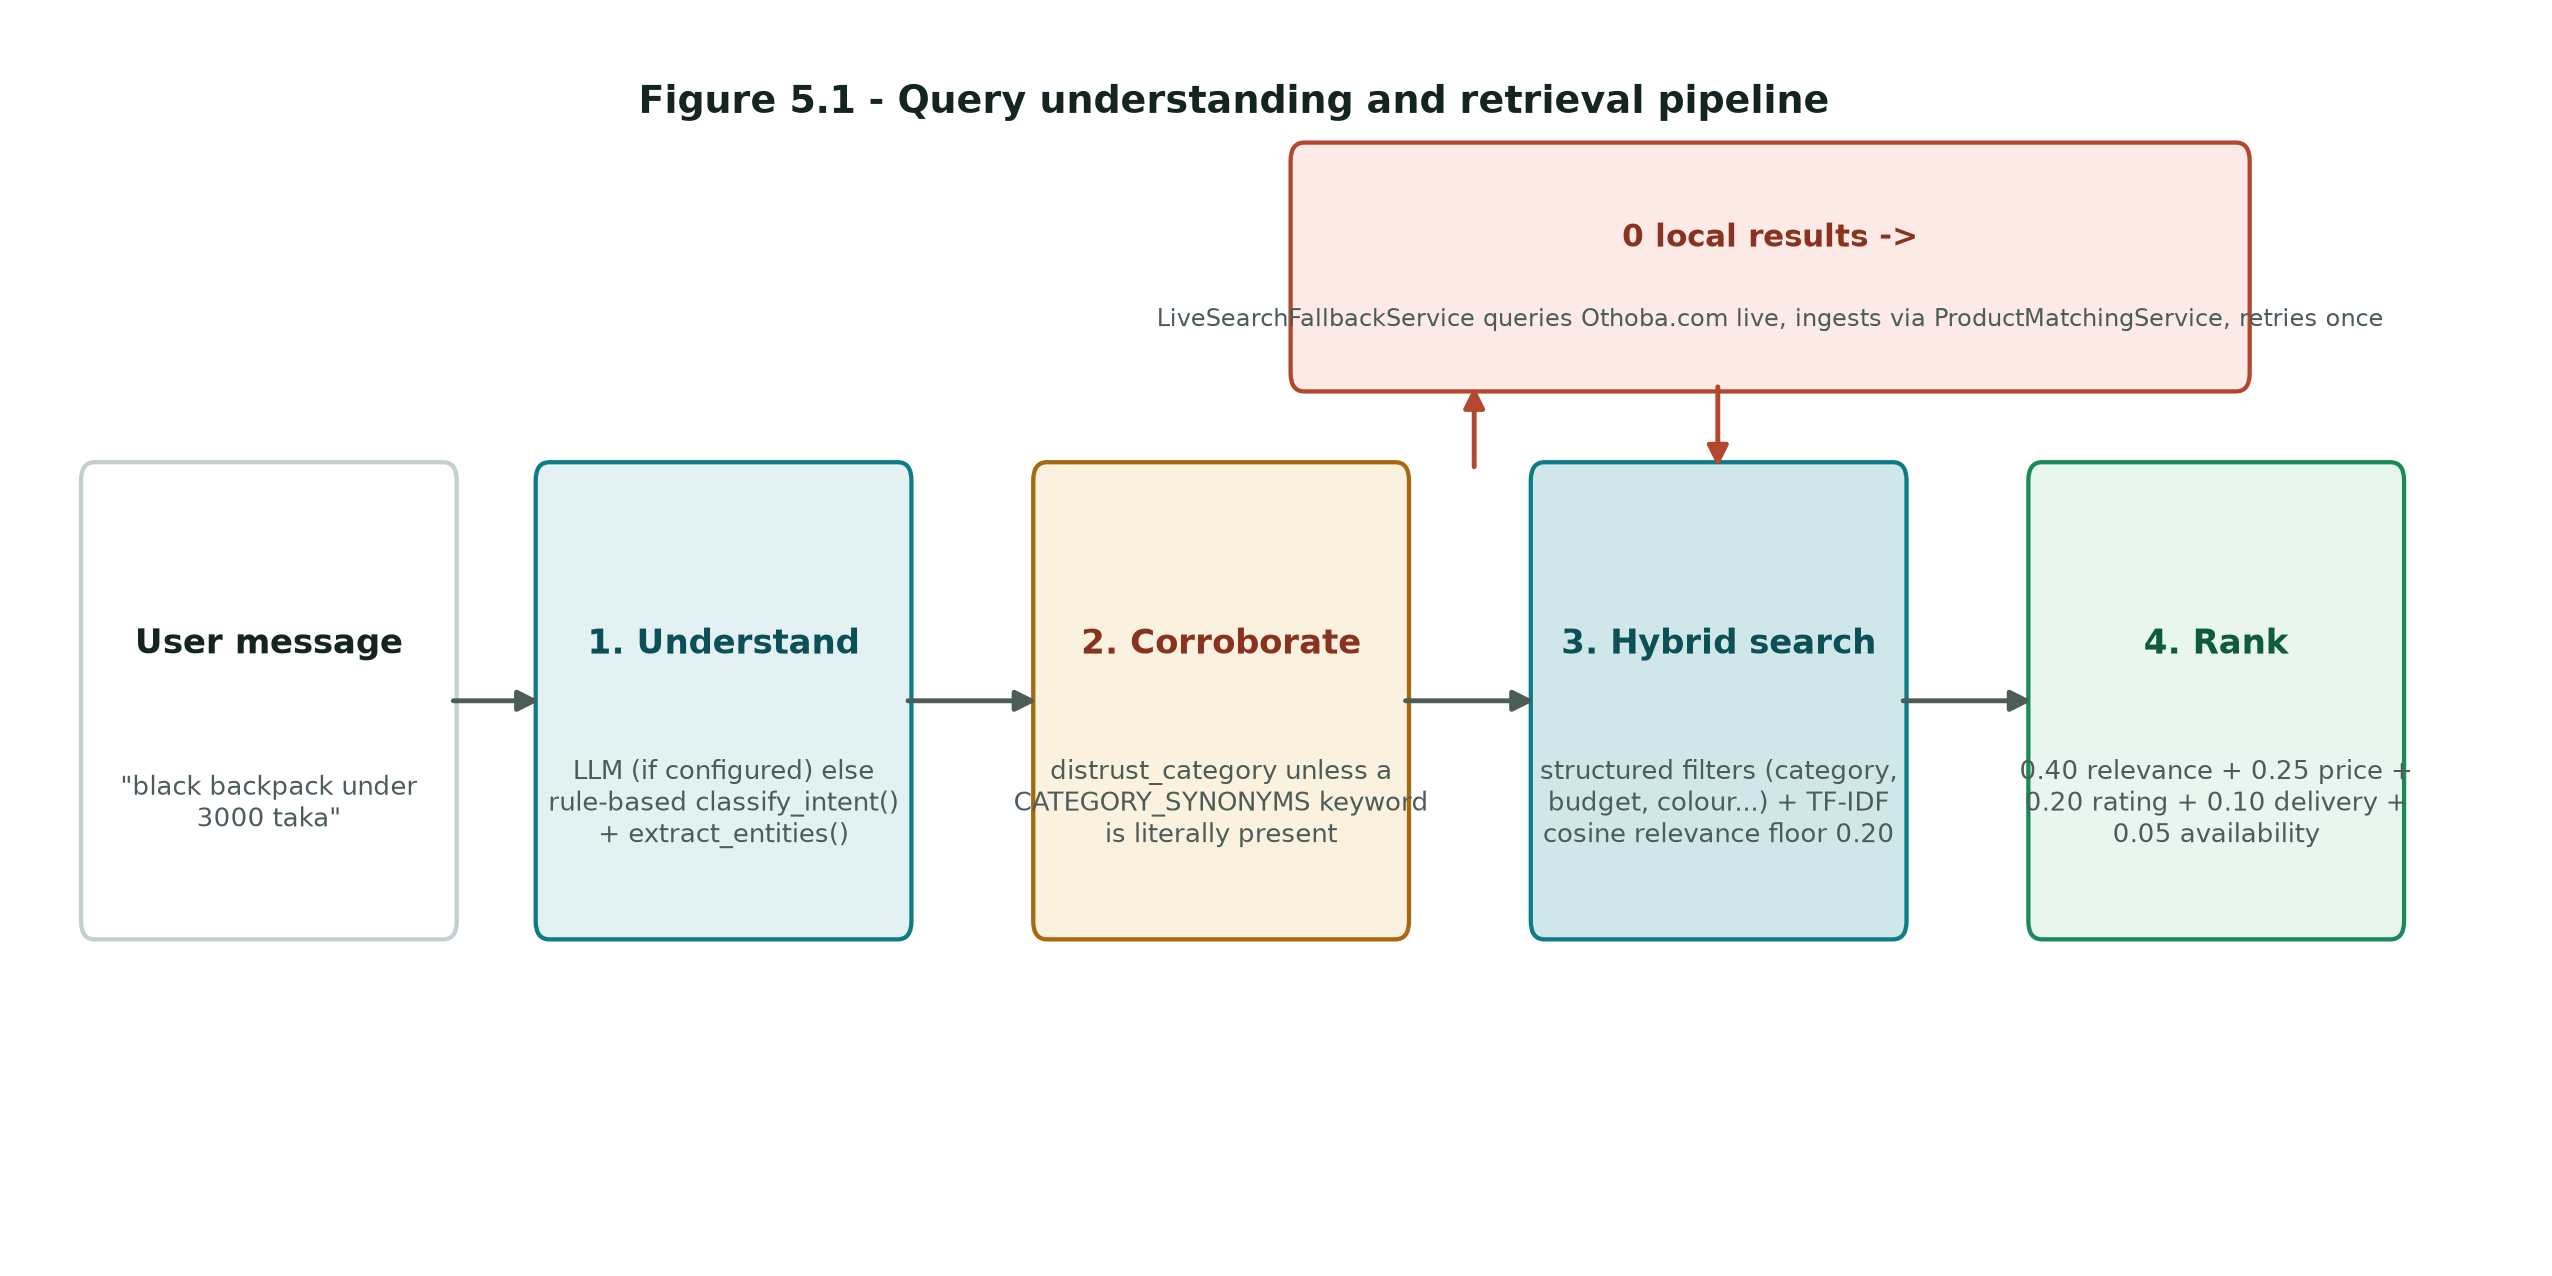
\includegraphics[width=0.98\textwidth]{fig_pipeline.png}
\caption{Query understanding and retrieval pipeline.}
\label{fig:pipeline}
\end{figure}

\section{Query Understanding: Rule-Based NLU}
The rule-based pipeline (\texttt{nlp.py}) is the system's deterministic baseline: it classifies intent by
checking the lower-cased message against per-intent keyword lists (e.g. ``compare''/``vs'' for
\texttt{COMPARE\_PRODUCT}, ``notify me''/``price drop'' for \texttt{PRICE\_ALERT}), defaulting to
\texttt{SEARCH\_PRODUCT} when none match. Entity extraction runs a \texttt{CATEGORY\_SYNONYMS} dictionary
(e.g. ``phone''/``mobile''/\bn{ফোন} $\rightarrow$ ``Smartphones''), a \texttt{COLOUR\_WORDS} dictionary
with Bangla entries (e.g. \bn{কালো}/``kalo'' $\rightarrow$ ``black''), a \texttt{KNOWN\_BRANDS} list, and
regular expressions for budget (``under 3000 taka'', ``3000 er moddhe'') and rating thresholds (``4+
star'', ``highly rated'').

Matching is whole-word, not substring: an early version used Python's \texttt{in} operator, which matched
``blue'' inside ``bluetooth'' and silently misfired the colour filter on every Bluetooth-related query.
Regex \texttt{\textbackslash b} word boundaries were tried next, but \texttt{\textbackslash b} is defined
in terms of \texttt{\textbackslash w}, which follows \texttt{str.isalnum()} --- and \texttt{isalnum()} is
\texttt{False} for Bangla vowel signs and the virama (the combining marks inside a word like \bn{কালো}),
so \texttt{\textbackslash b}\bn{কালো}\texttt{\textbackslash b} failed to match \bn{কালো} at all, since its
own trailing vowel sign read as a false word boundary. The final \texttt{\_word\_in()} helper checks the
actual neighbouring characters against Unicode category M* (combining marks) in addition to
\texttt{isalnum()}, which is correct for both scripts.

\section{Query Understanding: LLM Integration and Category Corroboration}
\texttt{nlp\_llm.py} is an optional, drop-in replacement for the rule-based pair, calling an
OpenAI-compatible chat-completions endpoint (a hosted gateway was used in evaluation runs; a local Ollama
\texttt{/v1} endpoint is equally supported) with a system prompt that constrains every field to the same
closed vocabulary \texttt{extract\_entities()} already uses --- the LLM cannot invent a category or colour
string that the retrieval layer would not recognise. \texttt{understand()} falls back to the rule-based
pair unconditionally on any failure: network error, timeout, non-2xx response, malformed JSON, or an
out-of-vocabulary field. This guarantees a misconfigured or unreachable LLM backend degrades chat to its
previous behaviour rather than breaking search.

A second, more subtle problem required an explicit fix. The rule-based pipeline's category is only ever
set from a literal \texttt{CATEGORY\_SYNONYMS} keyword actually present in the message, so the retrieval
layer could safely trust a non-empty category unconditionally. An LLM has no such constraint --- it can
place ``washing machine'' in ``Home Appliances'' on loose semantic association even when the catalogue has
no washing machines at all, which, unfixed, let the LLM narrow a search to a category with no genuine
match and return nothing useful. The fix, \texttt{\_category\_is\_corroborated()}, re-checks the LLM's
category against the same \texttt{CATEGORY\_SYNONYMS} dictionary the rule-based path trusts: if a literal
synonym keyword is present in the message for that exact category, the category is trusted exactly as much
as the rule-based pipeline always was; otherwise a \texttt{distrust\_category} flag is set and passed to
the retrieval layer (Section~5.3), which applies a stricter per-candidate relevance floor instead of an
outright rejection.

\codebox{%
def \_category\_is\_corroborated(message: str, category: str) -\/> bool:\\
\ \ text = message.lower()\\
\ \ return any(\\
\ \ \ \ mapped == category and \_word\_in(text, keyword)\\
\ \ \ \ for keyword, mapped in CATEGORY\_SYNONYMS.items()\\
\ \ )
}

\section{Hybrid Retrieval: Structured Filters + TF-IDF}
\texttt{hybrid\_search()} (\texttt{search.py}) first applies any structured entity filters --- exact
category and brand match, colour substring match on the product's attributes, and numeric
budget/rating/free-delivery filters against each store listing --- narrowing the catalogue to a candidate
set. If a structured filter was present but the candidate set is empty, the function returns immediately
with no results, rather than falling through to an unfiltered ranking of the whole catalogue (an early
version of this exact fallthrough was the system's first ``random results'' bug).

A \texttt{TfidfVectorizer} is then fit over the candidate titles/categories/brands/descriptions plus the
query, and cosine similarity against the query vector becomes each candidate's relevance score. Two
distinct situations can let TF-IDF surface coincidental word overlap as if it were a real match, and both
are guarded by the same per-candidate \texttt{MIN\_RELEVANCE\_FLOOR} (calibrated at 0.20 against this
catalogue, where genuine unconstrained matches such as ``Redmi Note 13'' $\rightarrow$ ``Xiaomi Redmi Note
13'' score $\geq$ 0.29 while coincidental overlap such as ``gaming console'' $\rightarrow$ a computer desk
tops out at 0.19):
\begin{itemize}
\item A fully free-text query with no structured entity at all, where every product is a default
candidate;
\item A structured category that came from the LLM and was not corroborated (Section~5.2).
\end{itemize}

\noindent The floor is applied per candidate, not to the whole result set at once --- an earlier version
rejected the entire candidate set whenever every member showed zero relevance, which meant a single
coincidentally-matching product let the whole wrong set through uncut (documented in the Section~6.5 case
study). The floor is also skipped for a query containing non-Latin letters (detected by codepoint~$>$
U+024F, past Latin Extended-B): the English-only catalogue can never show TF-IDF overlap with a
Bangla-script query regardless of whether the underlying match is correct, so applying a lexical floor
there would reject everything on a property of the query's language, not the match's correctness.

\section{Multi-Factor Ranking}
\texttt{rank\_products()} (\texttt{ranking.py}) computes, for each candidate, its best offer (the lowest
total cost among in-stock listings, or among all listings if none are in stock), then min-max normalizes
four signals across the candidate set --- total cost (reversed, so cheaper scores higher), rating,
delivery charge (reversed), and TF-IDF relevance --- plus a binary availability signal, and combines them
into a single weighted score:

\begin{table}[H]
\centering
\begin{tabular}{lc}
\toprule
\textbf{Signal} & \textbf{Weight} \\
\midrule
Relevance (TF-IDF) & 0.40 \\
Price (lower is better) & 0.25 \\
Rating & 0.20 \\
Delivery cost (lower is better) & 0.10 \\
Availability & 0.05 \\
\bottomrule
\end{tabular}
\caption{Ranking signal weights.}
\end{table}

\noindent The top-ranked results are then each assigned one human-readable reason --- ``Lowest price'',
``Best rated'', ``Fastest / cheapest delivery'', or ``Best overall match'' for everything else --- computed
directly from the same best-offer data used for scoring, so the stated reason for a recommendation is
never inconsistent with the numbers shown alongside it.

\section{On-Demand Live Search Fallback}
When \texttt{ChatController::send()} receives an empty result set from the AI service,
\texttt{LiveSearchFallbackService} issues a single live query against Othoba.com's public, search-only
Typesense endpoint for the exact typed message, ingests any genuine hits through the same
\texttt{ProductMatchingService} used for batch import (Section~4.5) --- so a live-fallback ingestion is
held to exactly the same brand/model-code vetoes as a scheduled import --- and then retries the original
AI-service query once. The retry passes back the already-resolved intent and entities so the AI service
can skip a second \texttt{understand()} round trip entirely; this optimization was measured to cut a
fallback-triggering query's total latency from 13.6 seconds to 5.8 seconds. The fallback never throws: any
failure (network error, empty live results) simply leaves the original empty result in place, and the
pre-order/notify-me flow (Section~5.6) remains available for genuinely absent products.

\texttt{OthobaLiveProvider} maps Othoba's own category text to ShopMate's taxonomy and prefers that mapped
category over a search-term-derived hint when it resolves to a known category. This fixed a real data bug
found during testing: batch imports seeded by a search term such as ``rice'' had tagged every hit ---
including an actual rice cooker, a kitchen appliance --- as Groceries, because the import pipeline had no
per-listing signal beyond the search term that produced it.

\section{Human-Confirmed Order and Notify-Me Workflow}
\texttt{OrderController::confirm()} shows a confirmation screen for one specific store listing (never
redirects automatically); only after the user submits that confirmation does
\texttt{OrderController::store()} record an order with status \texttt{confirmed\_redirected}. No payment
or checkout action is ever submitted to the store's own site --- the order row exists purely as ShopMate's
own record of confirmed intent, linking out to the store's real listing URL. When a search matches nothing
anywhere, including after the live fallback, \texttt{PreOrderController::store()} records the query,
category, and brand as a \texttt{pre\_order\_requests} row an administrator can act on manually --- the
same ``capture demand, act on it manually'' pattern used for the \texttt{possible\_duplicate\_products}
review queue (Section~4.3).

\section{Chat Interface: Responsiveness and Usability}
Two usability issues were fixed based on direct testing of the running application. First, a query that
reaches the AI service --- and especially one that triggers the live-fallback retry --- can take several
seconds; without a loading indicator, this read as an unresponsive page. The chat view now shows a
``thinking'' bubble and disables the send button for the duration of the request. The message input itself
is set read-only rather than disabled while the request is in flight: a disabled form field's value is
excluded from serialization, which would have silently stripped the just-typed message from the submitted
form data. Second, the chat view auto-scrolls to the latest message on load and after each reply, removing
the need to scroll manually through a growing conversation.

\section{Administrative Dashboard}
The admin dashboard (\texttt{AdminController}) summarizes store health (per-store listing counts and
last-checked timestamps), catalogue size, user counts, and recent search activity, with the
\texttt{possible\_duplicate\_products} and \texttt{pre\_order\_requests} queues surfaced for manual review
--- the operational counterpart to the automated matching and fallback pipelines described above.

% ============================================================
% CHAPTER 6
% ============================================================
\chapter{Testing and Evaluation}

\section{Research Question and Methodology}
\textbf{Research question:} can a conversational AI agent improve product discovery over conventional
keyword-based search on the category of query --- budget-aware, multi-constraint, and Bangla/Banglish ---
that a keyword index is structurally unable to resolve?

Eleven hand-labelled queries (\texttt{ai-service/eval/queries.json}) were designed to span six categories:
budget, budget+attribute (the project proposal's own worked example), brand, attribute/rating,
multi-constraint, Bangla/Banglish, and ambiguous-name ranking quality. Each query carries a ground-truth
set of relevant product IDs, hand-labelled against the fixed, pristine 20-product seeded catalogue produced
by the project's own \texttt{db:seed} command --- the same catalogue every re-run of
\texttt{eval/run\_evaluation.py} starts from, so the reported numbers are exactly reproducible.

The keyword-search baseline reproduces conventional single-platform e-commerce search: it matches literal
query tokens against product titles with no structured-constraint parsing, no cross-store matching, and no
language understanding beyond substring overlap. Both systems are scored on the same query set with
Precision@5, Recall@5, and NDCG@5 (Normalized Discounted Cumulative Gain) \cite{jarvelin2002}, computed by
\texttt{eval/run\_evaluation.py} directly against the rule-based \texttt{classify\_intent()}/
\texttt{extract\_entities()} pipeline --- never against the LLM pipeline --- specifically so the reported
numbers stay tied to a deterministic, reproducible component regardless of whether an LLM backend happens
to be configured when the evaluation is re-run.

\section{Results}
\begin{table}[H]
\centering
\begin{tabular}{lccc}
\toprule
\textbf{System} & \textbf{Precision@5} & \textbf{Recall@5} & \textbf{NDCG@5} \\
\midrule
ShopMate AI & 0.36 & 1.00 & 1.00 \\
Keyword baseline & 0.18 & 0.59 & 0.59 \\
\bottomrule
\end{tabular}
\caption{Mean Precision@5, Recall@5 and NDCG@5 over 11 evaluation queries.}
\label{tab:eval-summary}
\end{table}

\begin{longtable}{p{2.6cm}p{4.4cm}p{2.7cm}p{2.7cm}}
\caption{Per-query results (Precision@5 / Recall@5 / NDCG@5).}\label{tab:eval-detail} \\
\toprule
\textbf{Category} & \textbf{Query} & \textbf{ShopMate} & \textbf{Baseline} \\
\midrule
\endfirsthead
\toprule
\textbf{Category} & \textbf{Query} & \textbf{ShopMate} & \textbf{Baseline} \\
\midrule
\endhead
budget & backpack under 3000 taka & 0.6 / 1.0 / 1.00 & 0.6 / 1.0 / 0.91 \\
budget+attribute & black backpack under 3000 taka with a laptop compartment & 0.4 / 1.0 / 1.00 & 0.4 / 1.0
/ 0.92 \\
brand & Xiaomi products & 0.4 / 1.0 / 1.00 & 0.2 / 0.5 / 0.61 \\
attribute (rating) & highly rated wireless earbuds & 0.2 / 1.0 / 1.00 & 0.2 / 1.0 / 1.00 \\
budget & cheap phone under 22000 taka & 0.2 / 1.0 / 1.00 & 0.0 / 0.0 / 0.00 \\
multi-constraint & black smartphone with free delivery under 26000 & 0.4 / 1.0 / 1.00 & 0.0 / 0.0 / 0.00 \\
bangla/banglish & \bn{কালো ব্যাগ} & 0.6 / 1.0 / 1.00 & 0.0 / 0.0 / 0.00 \\
bangla/banglish + budget & \bn{ব্যাগ ৳3000} er moddhe & 0.6 / 1.0 / 1.00 & 0.0 / 0.0 / 0.00 \\
ambiguous-name & leather office bag & 0.2 / 1.0 / 1.00 & 0.2 / 1.0 / 1.00 \\
ambiguous-name & kettle & 0.2 / 1.0 / 1.00 & 0.2 / 1.0 / 1.00 \\
ambiguous-name & long lasting shoes for running & 0.2 / 1.0 / 1.00 & 0.2 / 1.0 / 1.00 \\
\bottomrule
\end{longtable}

\section{Discussion}
The baseline scores exactly zero on every budget-aware, multi-constraint, and Bangla/Banglish query in the
set (``cheap phone under 22000 taka'', ``black smartphone with free delivery under 26000'', \bn{কালো
ব্যাগ}, \bn{ব্যাগ ৳3000} er moddhe) --- precisely the category of query the research question asks about,
and precisely what a keyword index that treats ``under'', ``22000'' and ``taka'' as three more literal
tokens to match, rather than a numeric filter, cannot resolve. ShopMate AI's structured-entity extraction
(Sections~5.1--5.2) parses the budget, brand, colour and delivery constraints independently of the
free-text relevance score, so these queries resolve correctly regardless of whether any product title
happens to contain the literal query words.

Precision@5 is modest for both systems (0.36 for ShopMate, 0.18 for the baseline) not because ranking
quality is poor, but because most queries in this 20-product catalogue have only one to three truly
relevant products against a cut-off of K=5 --- an honest, stated limitation of evaluating against a small
seeded catalogue rather than a production-scale one, and the reason Recall@5 and NDCG@5 are the more
informative metrics here: ShopMate AI reaches perfect recall and ranking quality (1.00/1.00) on every query
in the set, meaning every genuinely relevant product was both retrieved and ranked at the top, while the
baseline's recall (0.59) and NDCG (0.59) reflect the queries it fails outright.

The one query category where both systems score identically (``highly rated wireless earbuds'', ``leather
office bag'', ``kettle'', ``long lasting shoes for running'' --- the ambiguous-name/ranking-quality
category) shows the two systems agreeing exactly when the query is a plain single-category lookup with no
budget, brand, or language constraint to resolve --- the case a keyword index is actually built for.

\section{Non-Functional Evaluation}
Beyond retrieval quality, two engineering properties were validated directly rather than through the
scored query set. Graceful LLM degradation (NFR-2) was verified by disabling the configured LLM endpoint
and confirming chat continued to function through the rule-based pipeline with no visible error. The
live-fallback latency optimization (Section~5.5) was measured directly: a fallback-triggering query's total
response time fell from 13.6 seconds (re-running full query understanding after ingestion) to 5.8 seconds
(retrying with the already-resolved intent/entities passed through).

\section{Engineering Case Study: Calibrating the Semantic-Trust Threshold}
This section documents a real, multi-round bug chain encountered while integrating the optional LLM
backend, because the fix illustrates a general principle --- distinguishing lexical evidence from semantic
correctness --- more clearly than an abstract description of the final design would.

\textbf{Round 1.} The original \texttt{hybrid\_search()} returned the entire catalogue, ranked, whenever a
structured filter matched zero candidates --- an unconstrained ranking pass over unrelated products
presented as search results. Fixed by returning an empty result immediately once a structured filter
yields no candidates.

\textbf{Round 2.} Adding the LLM backend reintroduced the bug through a different path: an LLM-supplied
category, unlike a rule-based one, is not guaranteed to correspond to anything the message literally said.
An initial fix rejected the whole result set whenever every candidate showed zero TF-IDF relevance --- but
this broke ``phone'' (the catalogue's own titles say ``Smartphone'', a token mismatch TF-IDF cannot
bridge) and every Bangla-script query (an English-only catalogue can never show lexical overlap with
Bangla, regardless of correctness).

\textbf{Round 3.} A substring-overlap check (``does any candidate share a substring with the query'')
fixed ``phone'' but not ``earphone'' (a true synonym, sharing no substring with ``Audio'' or ``earbuds''),
and reintroduced the original bug at a larger catalogue size: once the catalogue grew a ``Multi Purpose
Mixer Grinder Blender Machine'' listing, a ``washing machine'' query --- nothing genuine in the catalogue
--- coincidentally shared the word ``machine'' with that one Home Appliances product, and because the check
operated on the whole candidate set rather than per candidate, that one coincidental match let all 27
unrelated Home Appliances products through uncut.

\textbf{Final fix.} The trust decision was moved to where it belongs --- \texttt{nlp\_llm.py}'s
\texttt{\_category\_is\_corroborated()} (Section~5.2), checked against the same
\texttt{CATEGORY\_SYNONYMS} dictionary the rule-based pipeline already trusted --- combined with a
per-candidate, not whole-set, \texttt{MIN\_RELEVANCE\_FLOOR} in \texttt{search.py} (Section~5.3). This was
verified against every known case simultaneously: ``phone'', ``earphone'', ``headset'', Bangla queries,
``washing machine'' (correctly empty), ``rice cooker'' (correctly found once the category-normalization
fix in Section~5.5 also landed), ``noodles'', and the full Phase-6 evaluation baseline in Section~6.2. The
general lesson generalized from this case: a lexical-overlap signal (substring or TF-IDF score) and a
semantic-correctness signal (does this category actually apply) are not interchangeable, and conflating
them either rejects true positives the lexical signal cannot see, or admits false positives the semantic
signal alone would have caught.

% ============================================================
% CHAPTER 7
% ============================================================
\chapter{Results and System Walkthrough}

This chapter presents the working system directly, through screenshots captured from the running
application (Laravel + FastAPI, seeded and live-ingested catalogue), rather than mockups.

\section{Multi-Constraint Search in English}
The query ``black backpack under 3000 taka with a laptop compartment'' is parsed into a category (Bags), a
colour (black), and a budget ceiling (3000) simultaneously, and the response states the resolved intent
and entities above the ranked results, so the constraint parsing is visible to the user rather than a
black box.

\begin{figure}[H]
\centering
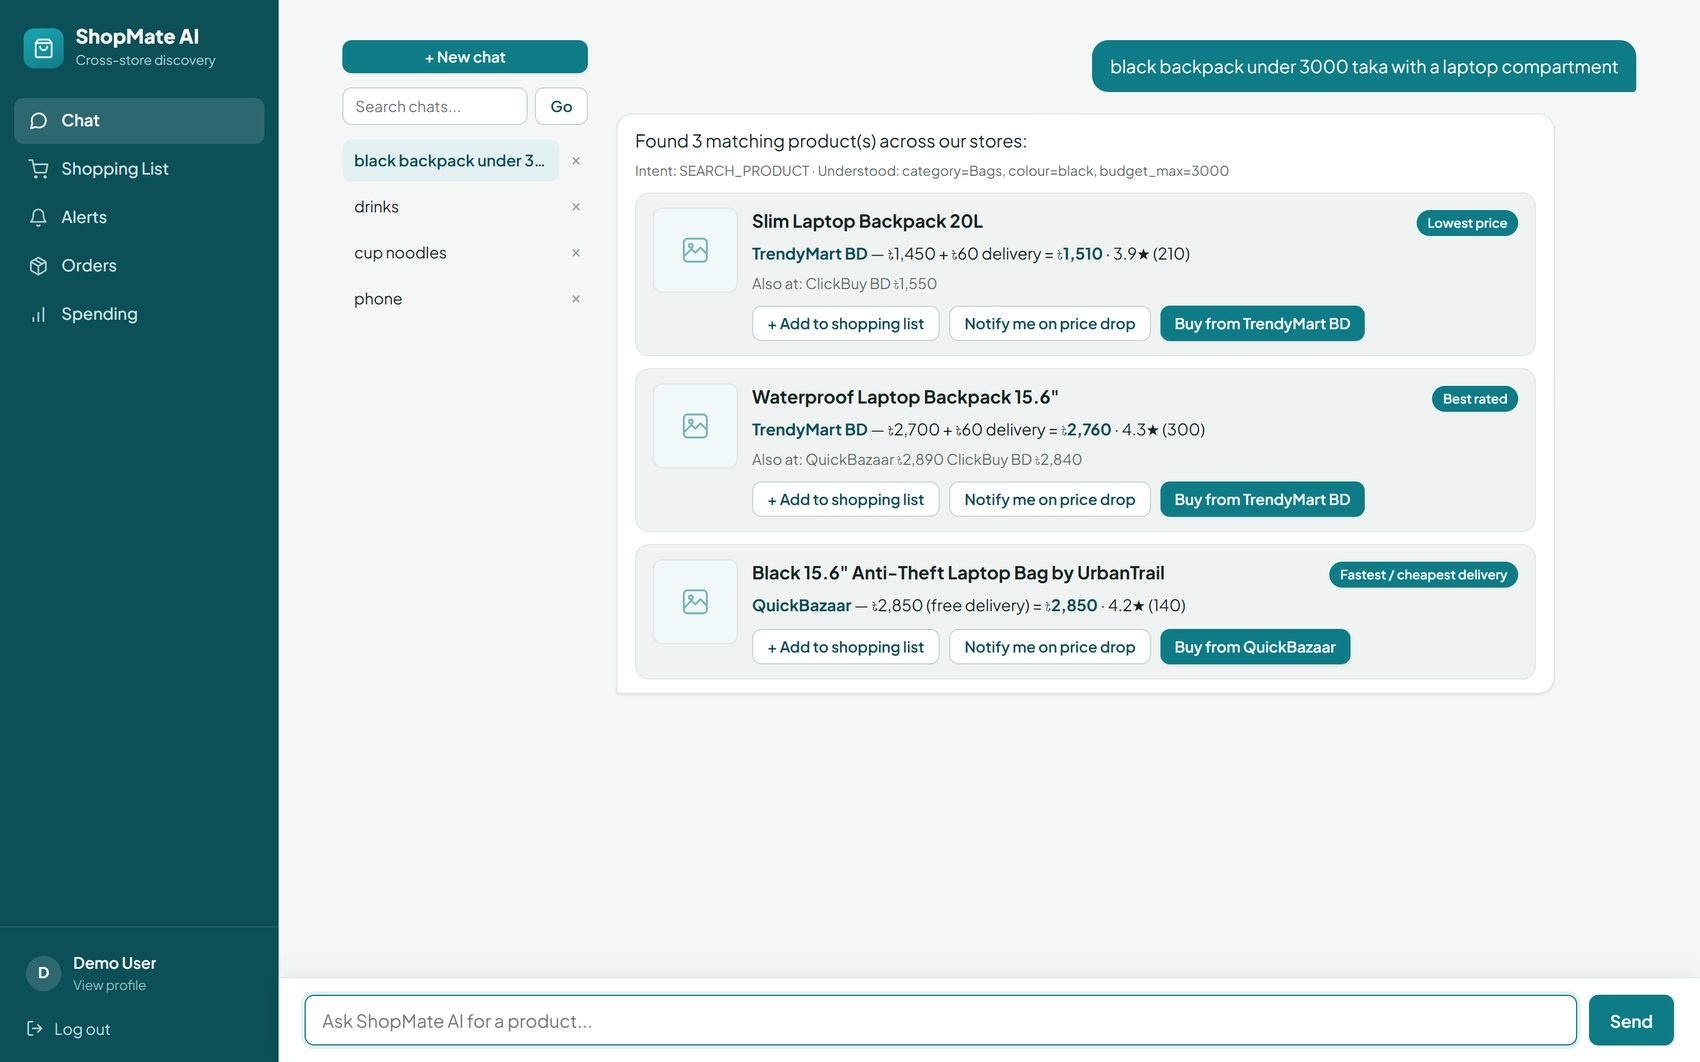
\includegraphics[width=0.86\textwidth]{01_chat_search_results.jpg}
\caption{English multi-constraint query: category, colour, and budget parsed and applied together.}
\end{figure}

\section{The Same Understanding in Bangla}
Within the same conversation, the Bangla query \bn{কালো ব্যাগ} (``black bag'') is understood identically
to its English equivalent and returns the same category of results, demonstrating that the entity
dictionaries (Section~5.1) and the non-Latin-aware relevance floor (Section~5.3) work together rather than
one silently defeating the other.

\begin{figure}[H]
\centering
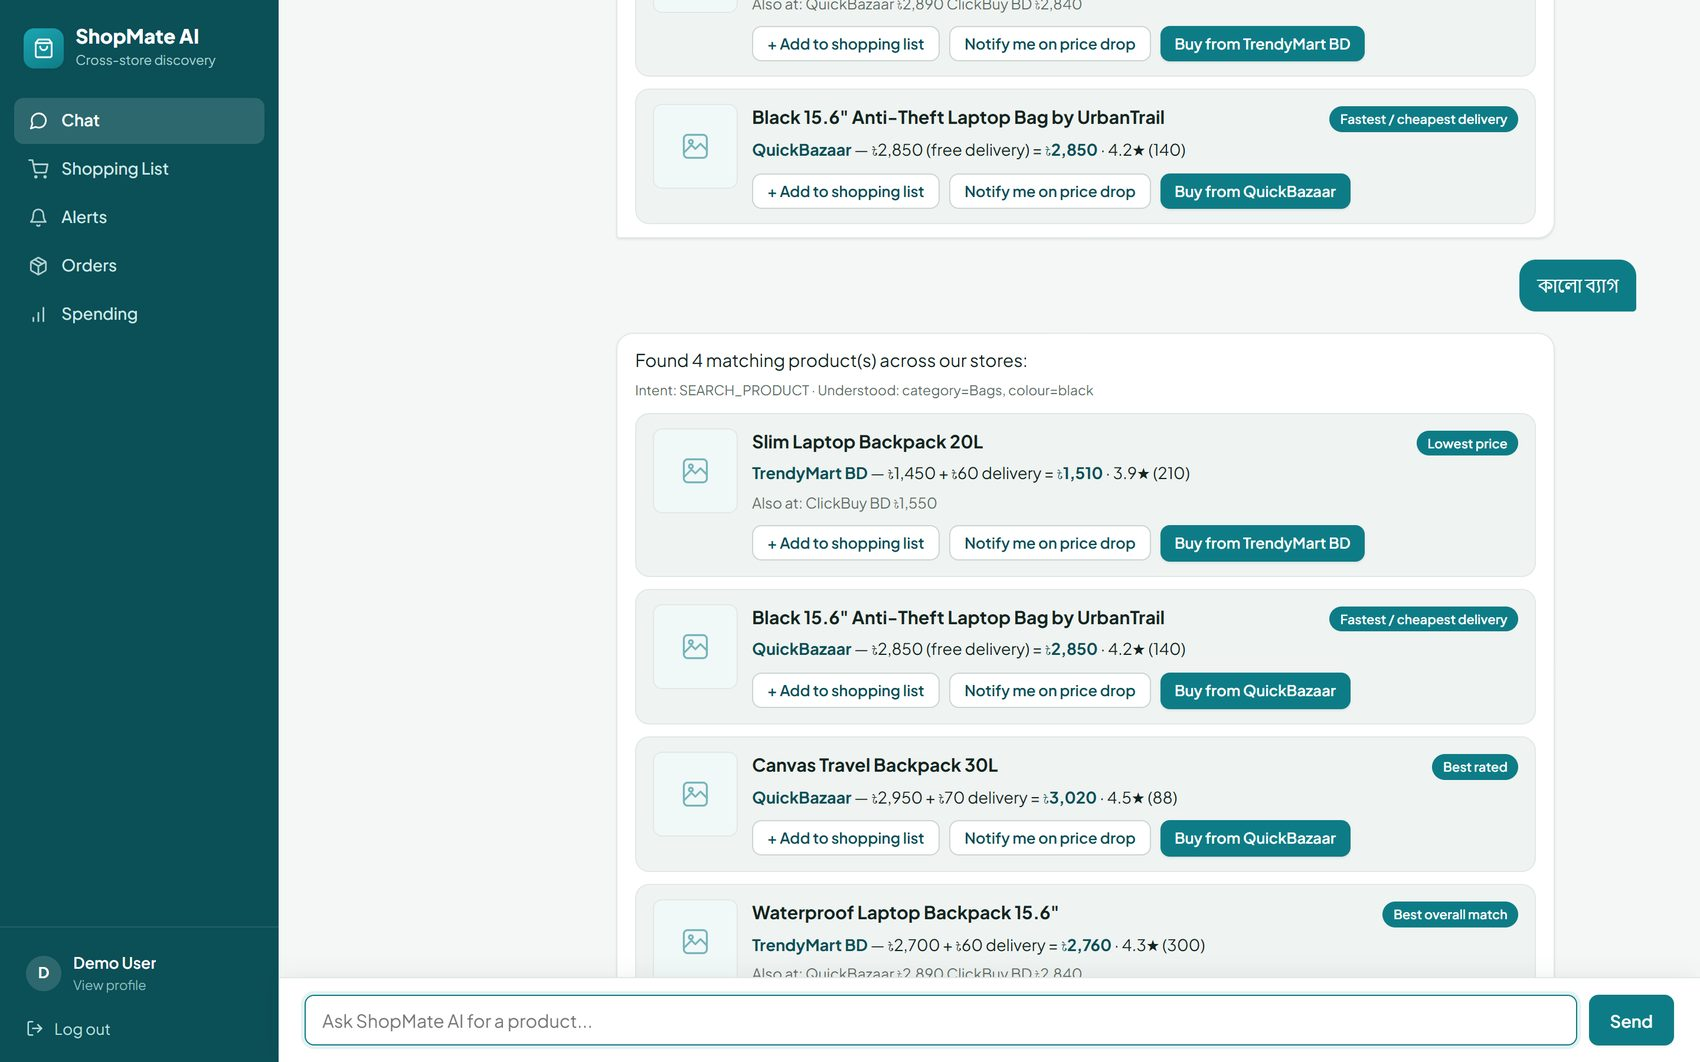
\includegraphics[width=0.86\textwidth]{02_chat_bangla_query.jpg}
\caption{Bangla-script query in the same session, understood and answered identically to its English
equivalent.}
\end{figure}

\section{A Genuinely Absent Product}
Searching for ``telescope for astronomy'' --- a product genuinely outside the seeded catalogue and outside
what the live-fallback search could find on Othoba.com --- correctly reports that nothing is available
rather than fabricating or coincidentally matching an unrelated result, and offers the pre-order/notify-me
path described in Section~5.6.

\begin{figure}[H]
\centering
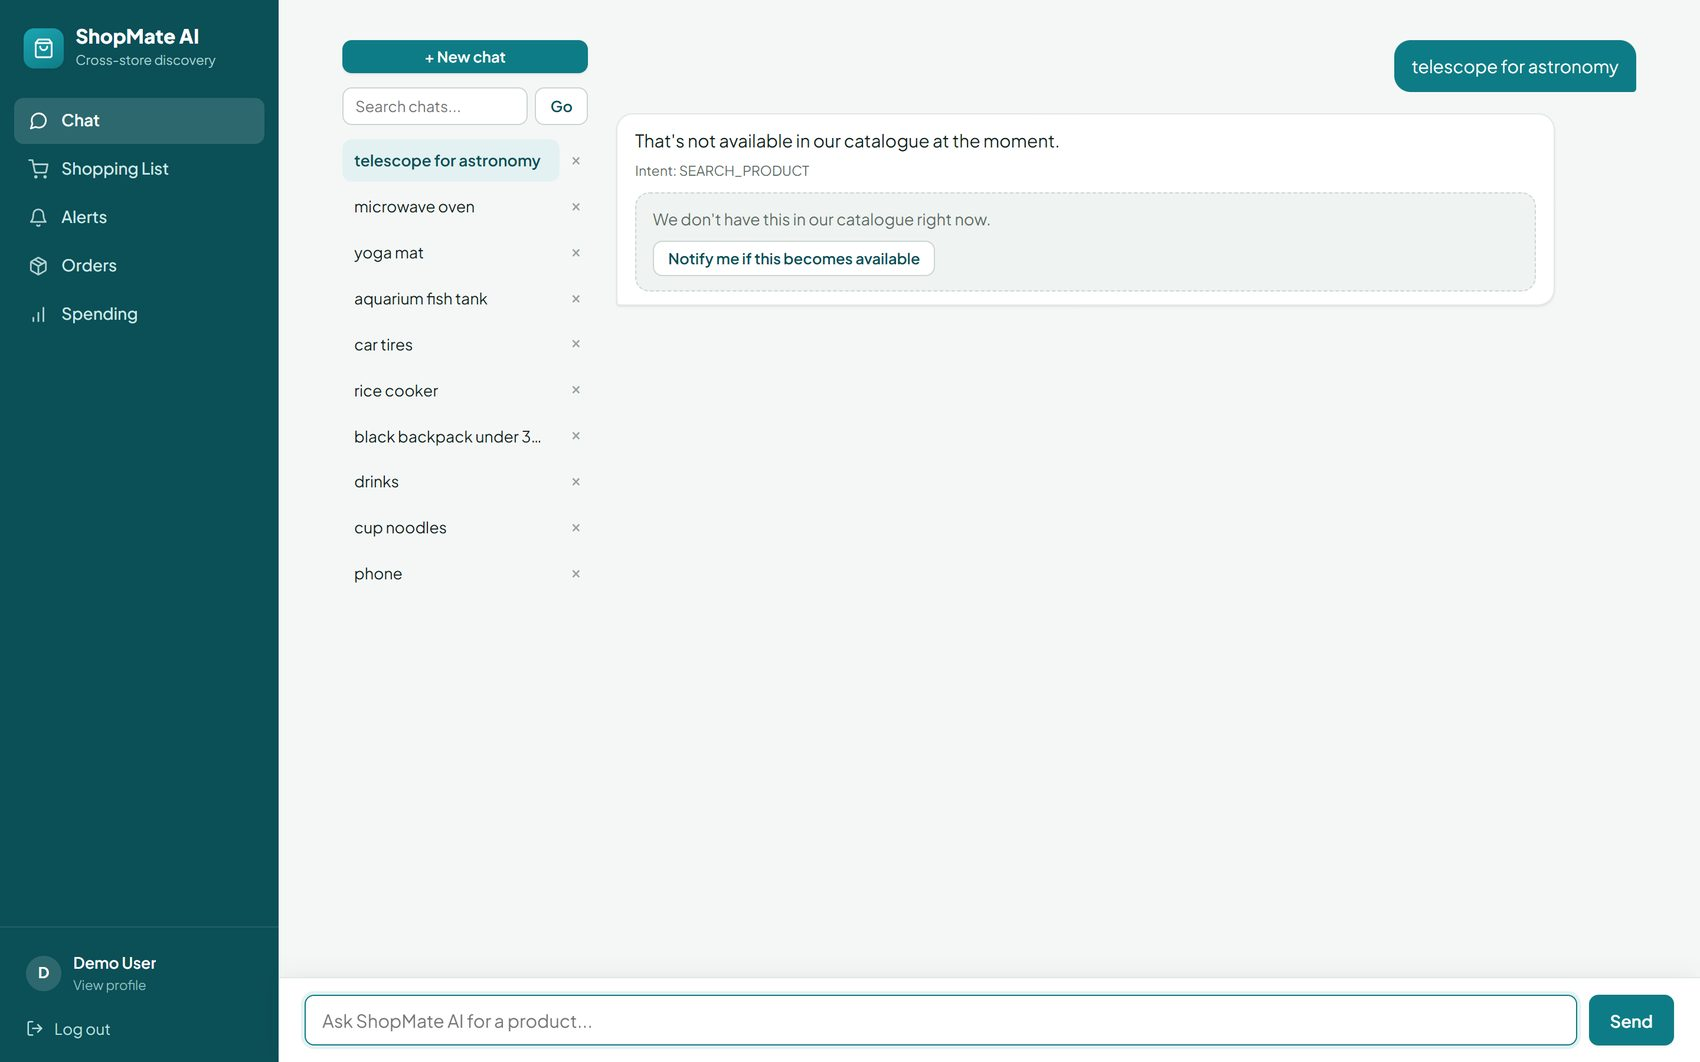
\includegraphics[width=0.6\textwidth]{03_chat_not_available.jpg}
\caption{A correctly-reported ``not available'' result, with a pre-order/notify-me option rather than a
fabricated match.}
\end{figure}

\section{Cross-Store Comparison from a Live-Ingested Product}
The order-confirmation screen below is for a rice cooker that ShopMate AI did not have in its seeded
catalogue at all --- it was found through the live-fallback search described in Section~5.5, correctly
categorised as Home Appliances (not Groceries) by the category-normalization fix in the same section, and
ingested as a new canonical product through \texttt{ProductMatchingService}. The confirmation step shows
the exact listing, its real price and delivery cost, and links out to the store's own page; no order or
payment is submitted anywhere until the user presses ``Confirm order'' here.

\begin{figure}[H]
\centering
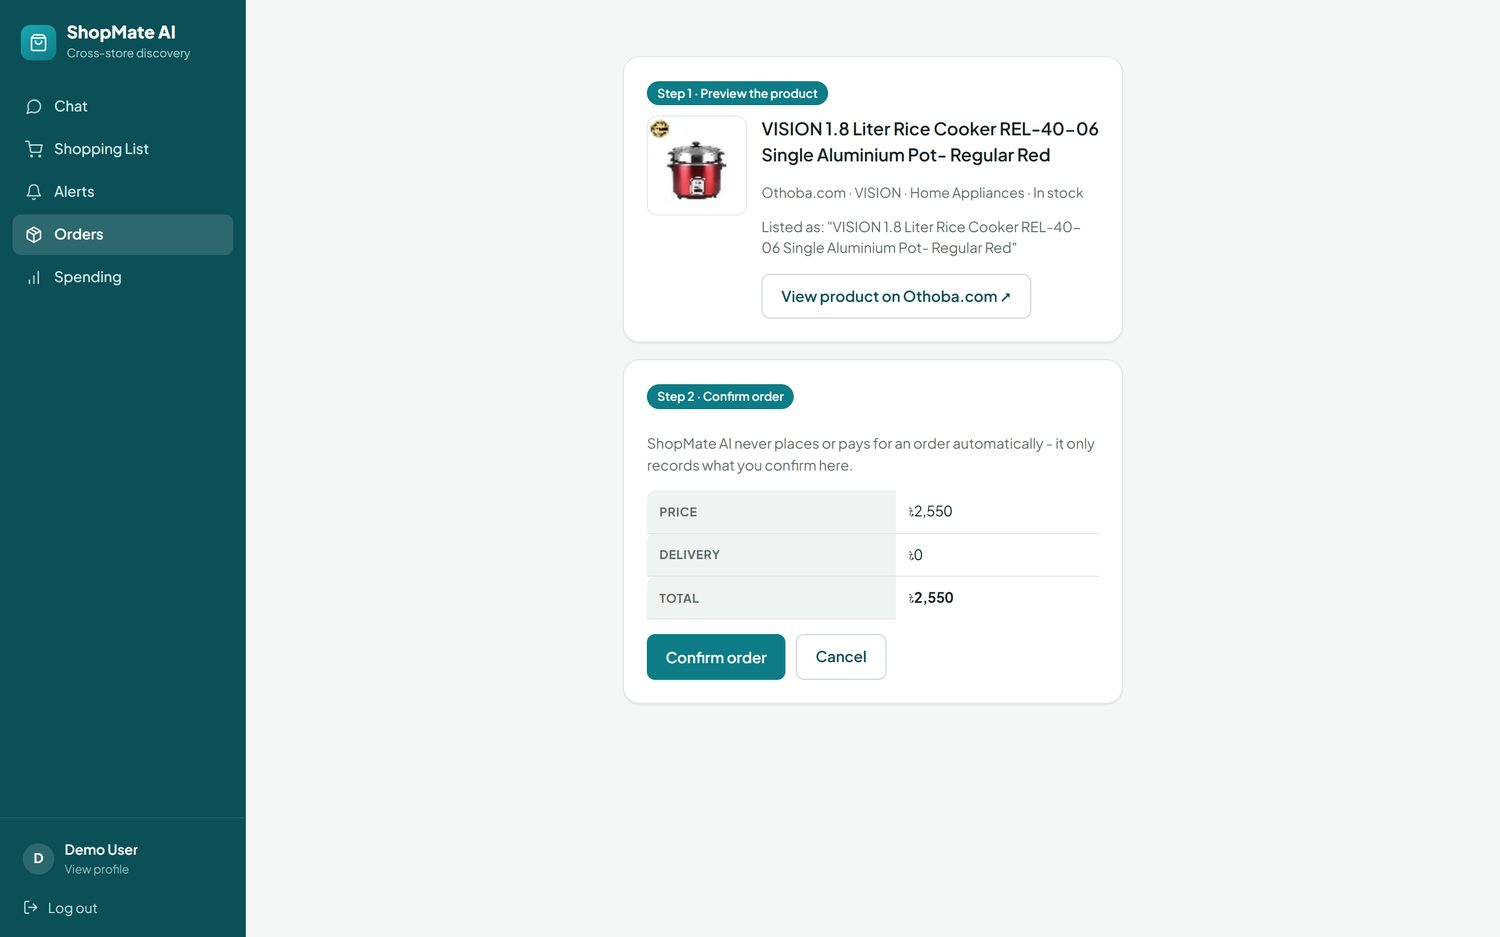
\includegraphics[width=0.55\textwidth]{04_order_confirm.jpg}
\caption{Human-confirmed order screen for a rice cooker discovered through the live-fallback search.}
\end{figure}

\section{Administrative Dashboard}
The admin dashboard reflects live catalogue and operational state --- at the time of capture, 284 products
across 5 stores, 2 users, 2 recorded orders, 9 logged searches, 0 outstanding pre-order requests, and a
mean AI-confidence (ranking score) of 0.729 across recent results. The ``Possible Duplicate Products''
queue lists pairs the matching service (Section~4.5) flagged as similar but below its auto-merge
threshold --- visible here are pairs such as two differently-branded Bluetooth earbud listings at 0.50
similarity and two ASUS VivoBook listings at 0.63 similarity, each awaiting a manual ``Merge'' or ``Not a
duplicate'' decision rather than being auto-merged on a borderline score.

\begin{figure}[H]
\centering
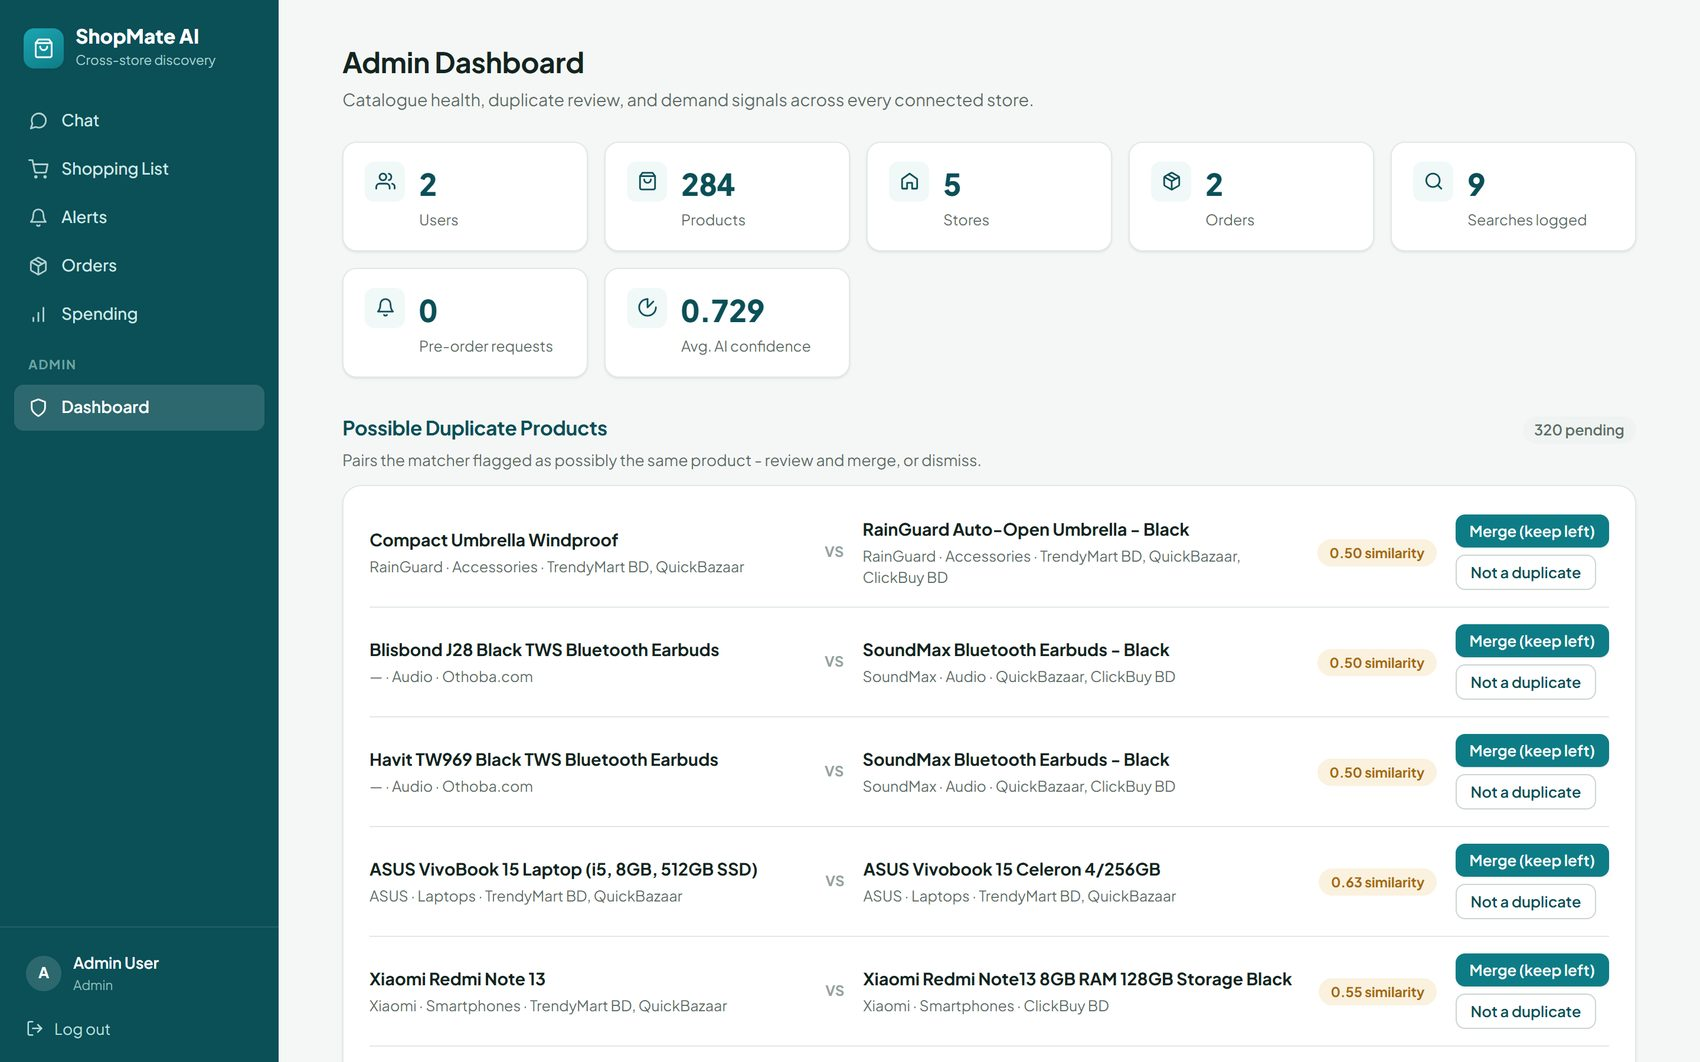
\includegraphics[width=0.92\textwidth]{05_admin_dashboard.jpg}
\caption{Admin dashboard: catalogue health, activity counters, and the manual duplicate-review queue.}
\end{figure}

\section{Spending Insights}
Beyond the modules in the original proposal (Section~4.3), a Spending Habits view was added during
implementation: it aggregates a user's own confirmed orders (Section~5.6) into total spend, order count,
average order value, a per-category breakdown, and a six-month trend, with short, data-driven
money-management tips generated from that same breakdown (e.g. flagging a shopping-list item with no
price-drop alert set).

\begin{figure}[H]
\centering
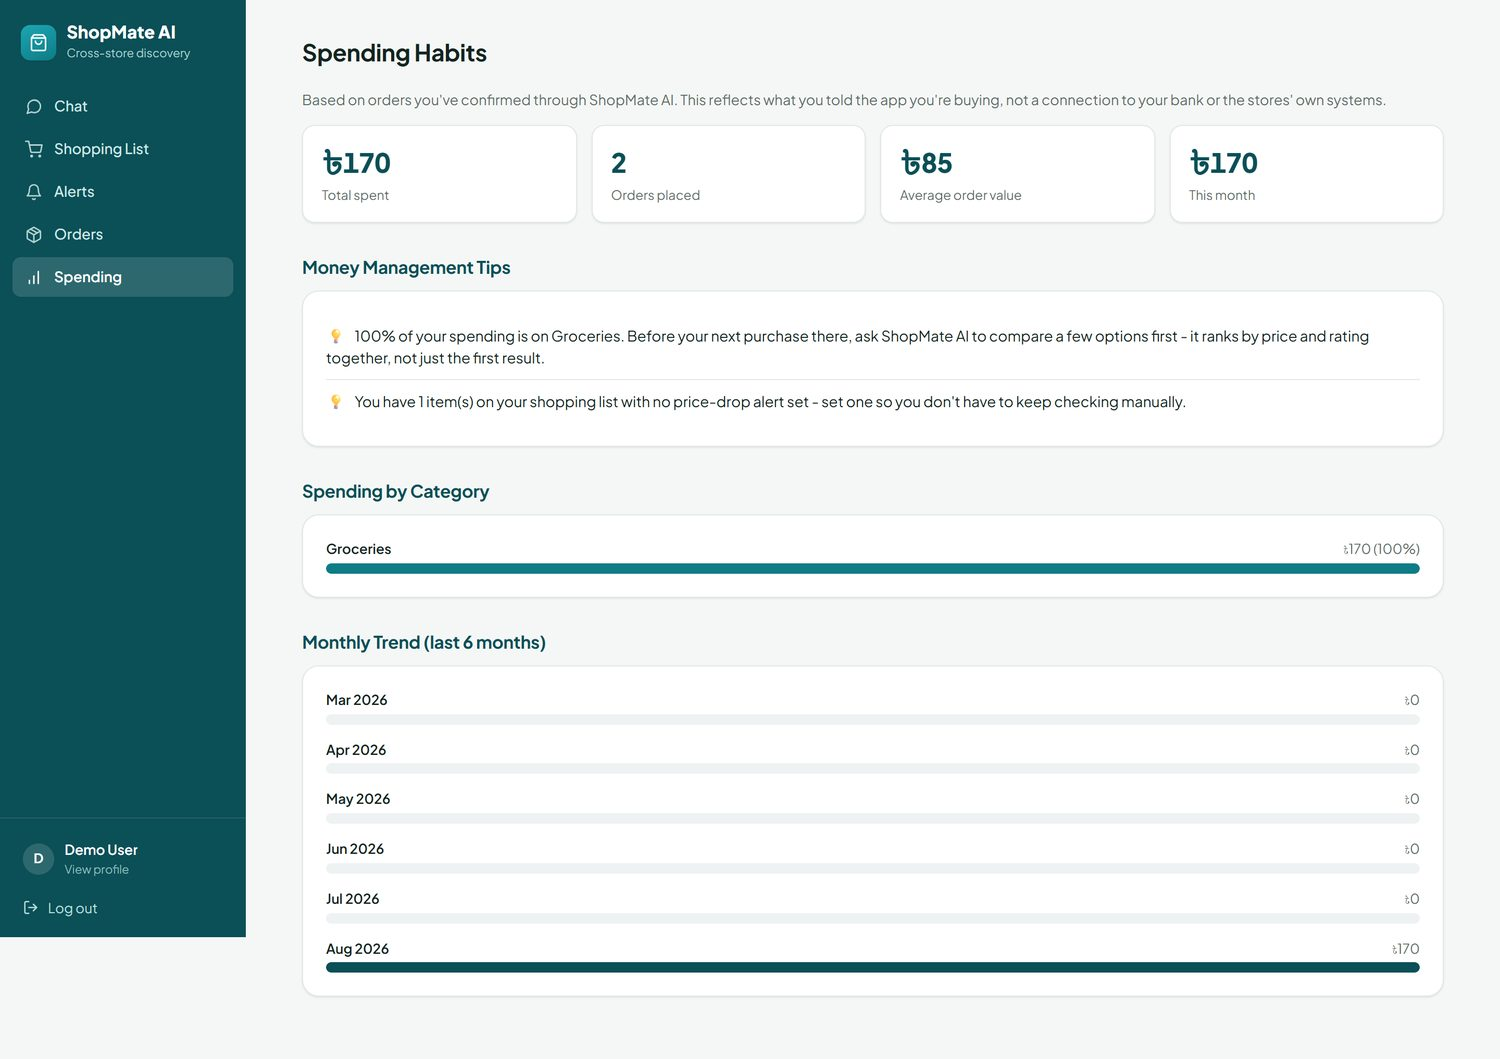
\includegraphics[width=0.8\textwidth]{06_spending.jpg}
\caption{Spending Habits view, derived entirely from the user's own confirmed orders.}
\end{figure}

% ============================================================
% CHAPTER 8
% ============================================================
\chapter{Conclusion and Future Work}

\section{Summary of Contributions}
\begin{itemize}
\item A working, service-oriented conversational shopping agent (Laravel + FastAPI) that separates
business logic from AI/NLP processing behind one internal API.
\item A dual-pipeline query-understanding system --- a deterministic rule-based extractor always
available, and an optional LLM backend whose every field is independently re-validated against the same
closed vocabulary, with unconditional fallback on failure --- plus a category-corroboration mechanism that
prevents an LLM's semantic over-reach from silently returning irrelevant results.
\item A hybrid TF-IDF and structured-filter retrieval pipeline with a calibrated, per-candidate relevance
floor, arrived at through a documented, multi-round debugging process (Section~6.5) that generalizes
beyond this project: lexical overlap and semantic correctness are different signals and must be checked
separately.
\item A dependency-free, two-veto cross-store product-matching service, tuned against both a clean fixture
and messy real listing data, that makes genuine multi-store price comparison possible rather than assumed.
\item An on-demand live-search fallback that extends catalogue coverage in real time and permanently
ingests genuine finds, with a measured latency optimization (13.6s to 5.8s) from skipping a redundant
language-understanding round trip on retry.
\item A human-confirmed order-recording workflow and a full evaluation against a conventional
keyword-search baseline, showing the experimental system reaches Recall@5~=~1.00 and NDCG@5~=~1.00 against
the baseline's 0.59 and 0.59, with the baseline scoring exactly zero on every budget-aware,
multi-constraint, and Bangla/Banglish query tested.
\end{itemize}

\section{Limitations}
\begin{itemize}
\item TF-IDF retrieval is a purely lexical signal; it cannot recognise a true synonym pair with no shared
substring unless that pair is already known to the \texttt{CATEGORY\_SYNONYMS} dictionary, which is why
the corroboration and relevance-floor mechanisms in Sections~5.2--5.3 exist as compensating controls
rather than a semantic model doing the work directly.
\item The evaluation catalogue is a fixed, seeded 20-product set; most queries have only one to three
truly relevant products against a Precision@5 cut-off, which is why Precision@5 is modest for both systems
even though ShopMate AI's recall and ranking quality are both perfect on this query set --- a larger,
production-scale catalogue would let Precision@K discriminate the two systems more sharply.
\item Live catalogue coverage depends on one real external integration (Othoba.com); broader live coverage
would require additional store adapters behind the existing \texttt{StoreProviderInterface}
(Section~4.4).
\item The cross-store matching threshold (0.65 / 0.80) was tuned against the store data available during
this project; a materially different catalogue (different marketing-boilerplate conventions, different
brand-naming patterns) would likely need re-tuning or a held-out validation set of its own.
\item Purchase actions are intentionally limited to human-confirmed recording rather than automated
checkout, by design rather than by omission (Section~1.5) --- this is a scope boundary, not a defect, but
it does mean the system does not itself complete a transaction.
\end{itemize}

\section{Future Work}
\begin{itemize}
\item Replace or augment TF-IDF retrieval with sentence-transformer embeddings once semantic
generalization beyond the synonym dictionary is needed, using the corroboration/relevance-floor pattern
from Sections~5.2--5.3 as the template for how to trust a semantic signal safely.
\item Add further store-provider integrations behind the existing \texttt{StoreProviderInterface} to
broaden live and batch catalogue coverage beyond Othoba.com.
\item Extend evaluation to a larger, production-scale catalogue and a real user study measuring task
completion time and subjective satisfaction, as outlined in the original project proposal's MSc
research-evaluation plan.
\item Explore a supported, official-API-based order-automation path for stores that offer one, strictly
preserving the human-confirmation requirement (Section~5.6) as a design invariant rather than relaxing it.
\item Apply active-learning to the \texttt{possible\_duplicate\_products} review queue (Section~7.5):
borderline matching decisions an administrator confirms or rejects could retune the Jaccard/threshold
parameters in Section~4.5 over time instead of leaving them fixed.
\end{itemize}

% ============================================================
% REFERENCES
% ============================================================
\begin{thebibliography}{99}

\bibitem{mikolov2013} T. Mikolov, I. Sutskever, K. Chen, G. Corrado, and J. Dean, ``Distributed
Representations of Words and Phrases and their Compositionality,'' in \textit{Advances in Neural
Information Processing Systems (NeurIPS)}, 2013, pp.~3111--3119.

\bibitem{reimers2019} N. Reimers and I. Gurevych, ``Sentence-BERT: Sentence Embeddings using Siamese
BERT-Networks,'' in \textit{Proc. EMNLP-IJCNLP}, 2019, pp.~3982--3992.

\bibitem{devlin2019} J. Devlin, M.-W. Chang, K. Lee, and K. Toutanova, ``BERT: Pre-training of Deep
Bidirectional Transformers for Language Understanding,'' in \textit{Proc. NAACL-HLT}, 2019,
pp.~4171--4186.

\bibitem{manning2008} C. D. Manning, P. Raghavan, and H. Sch\"utze, \textit{Introduction to Information
Retrieval}. Cambridge University Press, 2008.

\bibitem{jarvelin2002} K. J\"arvelin and J. Kek\"al\"ainen, ``Cumulated Gain-Based Evaluation of IR
Techniques,'' \textit{ACM Transactions on Information Systems}, vol.~20, no.~4, 2002, pp.~422--446.

\bibitem{owasp2021} OWASP Foundation, ``OWASP Top Ten Web Application Security Risks,'' 2021.
\url{https://owasp.org/www-project-top-ten/}

\bibitem{laravel} Laravel LLC, ``Laravel Documentation.'' \url{https://laravel.com/docs}

\bibitem{fastapi} FastAPI, ``FastAPI Documentation.'' \url{https://fastapi.tiangolo.com}

\bibitem{sklearn} scikit-learn developers, ``TfidfVectorizer --- scikit-learn Documentation.''
\url{https://scikit-learn.org/stable/modules/generated/sklearn.feature_extraction.text.TfidfVectorizer.html}

\bibitem{proposal} T. Ahmed, ``ShopMate AI --- Project Proposal: Design and Development of an
LLM-Orchestrated, Retrieval-Augmented Conversational Agent for Cross-Platform Product Discovery, Semantic
Product Matching and Personalized E-Commerce Recommendation,'' Mawlana Bhashani Science and Technology
University, 2026.

\end{thebibliography}
\addcontentsline{toc}{chapter}{References}

% ============================================================
% APPENDIX
% ============================================================
\appendix
\chapter{AI Service API Contract}
The AI service exposes a single endpoint consumed internally by the Laravel application.

\codebox{%
POST /chat/query\\
Content-Type: application/json\\[4pt]
\{\\
\ \ "message": "black backpack under 3000 taka with a laptop compartment",\\
\ \ "include\_international": false,\\
\ \ "intent": null,\\
\ \ "entities": null\\
\}
}

\noindent Response (truncated to one result):

\codebox{%
\{\\
\ \ "intent": "SEARCH\_PRODUCT",\\
\ \ "entities": \{\\
\ \ \ \ "category": "Bags", "brand": null, "colour": "black",\\
\ \ \ \ "budget\_max": 3000, "budget\_min": null,\\
\ \ \ \ "rating\_min": null, "free\_delivery": false\\
\ \ \},\\
\ \ "results": [\\
\ \ \ \ \{\\
\ \ \ \ \ \ "id": 1, "canonical\_title": "Slim Laptop Backpack 20L",\\
\ \ \ \ \ \ "category": "Bags", "brand": null, "score": 0.83,\\
\ \ \ \ \ \ "reason": "Lowest price",\\
\ \ \ \ \ \ "best\_offer": \{"store\_name": "TrendyMart BD", "price": 1450,\\
\ \ \ \ \ \ \ \ \ \ \ \ \ \ \ \ "delivery\_charge": 60, "total\_cost": 1510,\\
\ \ \ \ \ \ \ \ \ \ \ \ \ \ \ \ "rating": 3.9, "in\_stock": true\}\\
\ \ \ \ \}\\
\ \ ]\\
\}
}

\noindent \texttt{intent} and \texttt{entities} are accepted on the request specifically to support the
live-fallback retry (Section~5.5): when the Laravel controller re-calls this endpoint after ingesting new
listings for the same message, it passes back the already-resolved values so the service can skip
\texttt{understand()} entirely.

\chapter{Evaluation Query Set}
\begin{longtable}{p{2.6cm}p{3.6cm}p{6.4cm}}
\caption{Full evaluation query set (\texttt{ai-service/eval/queries.json}), 11 queries against the seeded
20-product catalogue.} \\
\toprule
\textbf{ID} & \textbf{Category} & \textbf{Query} \\
\midrule
\endfirsthead
\toprule
\textbf{ID} & \textbf{Category} & \textbf{Query} \\
\midrule
\endhead
budget-1 & budget & backpack under 3000 taka \\
budget-attr-1 & budget+attribute & black backpack under 3000 taka with a laptop compartment \\
brand-1 & brand & Xiaomi products \\
rating-1 & attribute (rating) & highly rated wireless earbuds \\
budget-2 & budget & cheap phone under 22000 taka \\
multi-1 & multi-constraint & black smartphone with free delivery under 26000 \\
banglish-1 & bangla/banglish & \bn{কালো ব্যাগ} \\
banglish-2 & bangla/banglish + budget & \bn{ব্যাগ ৳3000} er moddhe \\
ambiguous-1 & ambiguous-name & leather office bag \\
ambiguous-2 & ambiguous-name & kettle \\
ambiguous-3 & ambiguous-name & long lasting shoes for running \\
\bottomrule
\end{longtable}

\end{document}
